\documentclass[hidelinks]{scrartcl}
\usepackage{ngerman}
\usepackage[utf8]{inputenc}
\usepackage[ngerman,english]{babel}
\usepackage{amssymb}
\usepackage{graphicx}
\usepackage{fancyvrb}
\usepackage[mathbb]{}
\usepackage{amsmath}
\usepackage{amssymb}
\usepackage{float}
\usepackage{mathpazo}
\usepackage{listings}
\usepackage{pgfplots}
\usepackage{geometry}
\usepackage{upquote}
\usepackage{csquotes}
\usepackage{pdfpages}
\usepackage{colortbl}
\usepackage{rotating}
\usepackage{url}
\usepackage{hyperref}
\usepackage[nottoc]{tocbibind}
\usepackage[nomain,acronym,toc]{glossaries}
\loadglsentries{glossary}
\makeglossaries
\makeindex
\usepackage[round]{natbib}
\bibliographystyle{plainnat}
% For table highlighting and rotating of cells
\definecolor{Gray}{gray}{0.9}
\newcolumntype{g}{>{\columncolor{Gray}}c}
\newcommand*\rot{\rotatebox{90}}
\hyphenation{DaStruct}
\hyphenation{PRISM}
\setlength\parindent{0pt}

\begin{document}

\includepdf[pages={1-}]{titlepage}

\section*{Abstract}
Relational reasoning describes the spatial relationships between objects. When evaluating human performance in these tasks, some trends and preferences seem apparent. To explain these, computational implementations emulating humans are used. Previous implementations only used one specific combination of data structure and data method. To test which data structures and methods are most promising for predicting the difficulty of relational reasoning tasks for humans and for explaining the human relational reasoning process, a new computational implementation was written and the dependencies between data structures, methods and human performance were tested. \\
Two experiments were designed and carried out: One experiment measured the relationship between difficulty measures and the percentage of participants in an experiment able to solve a problem. The experiment showed that using a list-like data structure with a very low limit (i.e.\ only admitting two \gls{token}s) most reliably predicted how difficult a problem was for humans to solve. Also, the sum of model operations was a better predictor of difficulty than the sum of all difficulty measures. \\
A second experiment matched each participant to a specific combination of data structures and methods. The experiment showed that binary search tree data structures best match what actually happens in human heads. Some individuals clearly used binary search tree-like data structures limited in depth. The experiment suggests the existence of two main categories of reasoners.

\newpage
\section*{Zusammenfassung}
\begin{otherlanguage}{ngerman}
Relational reasoning beschreibt die räumliche Anordnung von Objekten. Die Auswertung menschlicher Leistung in Aufgaben zum relational reasoning weist bestimmte Charakteristika auf. Um diese zu erklären, werden Computerimplementationen genutzt, die menschliches Denken emulieren. Frühere Implementationen nutzten nur eine spezifische Kombination von Datenstruktur und -methode. Um herauszufinden, welche Datenstrukturen und -methoden am ehesten die Schwierigkeit, die eine relational reasoning Aufgabe für Menschen hat vorhersagen und welche Datenstrukturen und -methoden am ehesten dem menschlichen Modellierungsprozess entsprechen, wurde ein neues Programm geschrieben und die Beziehungen zwischen Datenstrukturen, -methoden und menschlicher Leistung analysiert. \\
Zwei Experimente wurden entworfen und durchgeführt: Ein Experiment maß die Beziehung zwischen Schwierigkeitsmaßen und dem Prozentsatz von Teilnehmenden an einem Experiment, die in der Lage waren, ein Problem richtig zu lösen. Das Experiment zeigte, dass eine listenähnliche Datenstruktur mit einer sehr niedrigen Beschränkung (also mit nur zwei beinhalteten Objekten) am zuverlässigsten vorhersagte, wie schwierig ein Problem für die Teilnehmenden war. Außerdem war die Teilsumme von Modell-Operationen ein besserer Prediktor als die Gesamtsumme aller Schwierigkeitsmaße. \\
Ein zweites Experiment wies jedem Teilnehmer eine spezifische Kombination von Datenstruktur und -methoden zu. Das Experiment zeigte, dass das menschliches Modellierungsverhalten am ehesten dem von Binärbäumen entspricht. Viele Teilnehmer nutzten eindeutig binärbaumähnliche Datenstrukturen, die in ihrer Tiefe beschränkt waren. Fast alle Teilnehmer nutzten eine von nur zwei verschiedenen Modellierungsstrategien.
\end{otherlanguage}

\newpage
\tableofcontents

\newpage
\section{Definitions}
\begin{itemize}
	\item A \textbf{premise} is a statement. In this thesis, premises are of the form ``A left B'' and denote that token A is situated to the left of token B.
	\item A \textbf{token} is an object that a premise or conclusion refers to. E.g. in the premise ``A left B'', A and B are tokens.
	\item A \textbf{conclusion} is a statement of the same form as a premise. In this thesis, conclusions are of the form ``A left B'' and denote that token A is left of B. Conclusions are checked for truth, i.e. in a model that has previously been built from premises, the validity of a conclusion is checked and returned.
	\item A \textbf{mental model} is a model representation of e.g. spatial information that is constructed by a person.
	\item The \textbf{working memory} is the part of human memory between sensory information and long term memory. Information 	that is to be included in long term memory is selected here, so the working memory acts as a sort of 			buffer. According to \cite{Baddeley.2007} it is divided into three subcomponents, one of which is the 		visuospatial sketchpad, which is responsible for storing visual and spatial information. Working 			memory has limited capacity, \cite{Miller.1956}'s law states that this capacity is 7 $\pm$ 2, i.e.\ any 		individual can keep about 7 objects concurrently in their working memory.
\end{itemize}
\newpage

\section{Introduction (or The Cave of Mysterious Monsters)}\label{sec:introduction}
Imagine entering a mysterious cave. There are four doors, each with a combative animal behind it. You must choose a door to advance. Luckily, there's a clue:
\begin{itemize}
\label{item:initial_problem}
\item The polar bear is left of the python.
\item The alligator is right of the python.
\item The cuddly kitten is left of the python.
\end{itemize}

\begin{figure}[!ht]
	\caption{Mysterious doors}
	\label{fig:mysterious_doors}
	\centering
	\includegraphics[width=0.7\textwidth]{Illustrations/choosing_door.jpg}
\end{figure}

Obviously, fighting against pythons, alligators and polar bears is difficult (for different reasons). You may want to choose the door with the kitten behind it. Which one is that? \\

If you only had little time to decide and no particular love for logic and statistics, it's likely that you'd choose the leftmost door. In fact, most people would do that.
\footnote{I guess. All people I personally asked was either confused by the contrived scenario or, perhaps due to their being computer science students, immediately convinced that this was Monty Hall and they had to ``switch to the other door''. Luckily, \cite{Ragni.2013} tested this experimentally.}  \\

This thesis is not (only) about human irrationality, but about spatial or \textit{relational reasoning}. Humans are born into and move through space all their life. The question of how objects are positioned in that space plays a crucial role in the ability of humans to stay alive and not constantly bump into walls. \\ Giving directions (``Turn left at the intersection immediately after the bank.''), information about where objects are located (``The box is on the table beneath the window in the room to your left.'') or remembering positions (``The quote was in the blue book on a right page somewhere at the end of the book.'') all involve relational reasoning: The ability to understand relative information as given in these sentences, interpret it correctly and — ideally — finding the object in question. \\
According to \cite{Baddeley.2007}'s model of \gls{working memory}, relational reasoning has its own dedicated space in human working memory: the so-called \textit{visuospatial sketchpad}. It holds visual and spatial information and allows mental manipulation thereof. \\

\noindent So, relational reasoning is:
\begin{itemize}
\item taking in information about space and objects in that space, 
\item taking in information about relationships between those objects and
\item drawing conclusions from this information.
\end{itemize}

The question of \textit{how} exactly to model human relational reasoning on a computer motivates this thesis.

\section{Model theory}\label{sec:model_theory}
Since people are able to give relations such as ``The python is left of the alligator'', when given the information from the introduction, they are obviously able to derive relations that were not explicitly given in the premises (i.e.\ deduce information). One possible way to build inferences could be by logical rules, e.g. for the transitivity \footnote{A relation is transitive ``if whenever an element a is related to an element b, and b is in turn related to an element c, then a is also related to c.'' \citep{Wikipedia.Transitive}} of relations. If \textit{A is left of B} and \textit{B is left of C}, then \textit{A is left of C}, by a simple logical rule. \\
However, this thesis is based on another way to understand human reasoning: \textit{The general theory of mental models} by \cite{Johnson-Laird.1986}. As summarized by \cite*{Jahn.2007}:

\begin{displayquote}
The theory of mental models, or the model theory for short, postulates that individuals use the meaning of assertions and general knowledge to construct models of the possibilities compatible with assertions.
\end{displayquote}

So what is stored in \gls{working memory} is not the information itself (e.g.\ as verbal representations of the premises), but a \textit{constructed mental model} that represents the given information.

\cite{Goodwin.2005} extend the general theory of mental models to describe the domain of relational reasoning by introducing the \textit{model theory of relational reasoning}\footnote{This model theory is not to be confused with this model theory: \url{https://en.wikipedia.org/wiki/Model_theory}}. They state that
\begin{itemize}
\item models used for relational reasoning are structurally iconic, i.e.\ the relations holding between the represented tokens are present between modeled tokens as well,
\item relational consequences are derived both from given relational information and general knowledge,
\item individuals construct only one, typical model and
\item ``the difficulty of an inference depends on the process of integration of the information from separate premises, the number of entities that have to be integrated to form a model, and the depth of the relation''.
\end{itemize}

There is considerable evidence for reasoners reasoning according to the model theory for relational reasoning problems \citep{Schaeken.2007}. \\

% For abstract: Information is not represented  visually "as is", but a representative internal mental model is created.

In the case of this thesis spatial information is given in the form of premises. One example for a set of premises can be found in the introduction (see section \ref{item:initial_problem}). Individuals iteratively construct models out of the premises, i.e.\ they build one or more models which may be increased and changed to represent all premises. Individuals use these models to draw conclusions and determine relationships between tokens mentioned in the premises. \\

\citet{Johnson-Laird.1991} separate the relational reasoning process into three phases:
\begin{itemize}
\item The \textit{comprehension phase}, named the \textit{model construction phase} by \cite{Ragni.2013}, in which reasoners construct a model from given information and forget the wording of the premises,
\item the \textit{description phase}, named the \textit{model inspection phase} by \cite{Ragni.2013}, in which reasoners inspect the mental model to derive relations that also hold but were not explicitly given in the premises and
\item the \textit{validation phase}, named the \textit{model variation phase} by \cite{Ragni.2013}, in which reasoners try all alternative models to see if one exists in which the conclusion they came to doesn't hold.
\end{itemize}

\noindent Even though the mental models are constructed individually, within one person, they seem to be quite predictably constructed and both stable
\begin{itemize}
\item within a population, i.e. most people construct the same internal mental model \citep{Ragni.2013}, \citep{Knauff.2013}, \citep{Rauh.2005}
\item as well as within an individual, i.e.\ one person constructs one mental model. \citep{Goodwin.2005}
\end{itemize}

\subsection{Inter- and Intrapersonal Stability of Mental Models}
To explain these stabilities, let's turn to the thesis advisor's work. One key idea of \cite{Ragni.2013} is the \textit{preferred model theory}.

\begin{displayquote}
A crucial assumption within our preferred model theory is that, in most situations, people only construct a single, simplified, and typical mental model and ignore all others. People are almost blind to alternative interpretations of the premises. We might only construct further models if the reasoning problem clearly requires us to consider alternatives. In other words, we do not think that the construction of an initial model is a stochastic process that produces one model this time and another the next time. In the preferred model theory, the construction of the initial model is, in principle, a deterministic process that always produces the same model for the same premises. We assume that this preferred model is the same for most people and that such preferred models bias people in a predictable way [...]. \\
\citep{Ragni.2013}
\end{displayquote}

Given the example from the introduction (see section \ref{sec:introduction} for the premises) it is both possible that the kitten is behind the first door and the polar bear behind the second,
\begin{figure}[H]
	\caption{Kitten, Polar bear, Python, Alligator}
	\label{fig:one_ordering}
	\centering
	\includegraphics[width=0.8\textwidth]{Illustrations/doors_animals_1.png}
\end{figure} 

as well as vice versa: The polar bear behind the first door and the kitten behind the second.
\begin{figure}[H]
	\caption{Polar bear, Kitten, Python, Alligator}
	\label{fig:different_ordering}
	\centering
	\includegraphics[width=0.8\textwidth]{Illustrations/doors_animals_2.png}
\end{figure}

When receiving new information as to what else is to the left of the python, besides the polar bear, there's a choice of ``where to put that information''. One possibility is to leave the previously constructed model of ``Polar bear, Python'' intact and to add a kitten to the left of that. The other possibility is to move the polar bear further to the left so that there's space for the kitten to crawl in between polar bear and python. \\
However, ``the preferred model is favored over others because it is easier to construct in spatial working memory'' \citep{Ragni.2013}. Moving items seems to be more work, since a moving operation requires the polar bear to be held in an extra slot, then adding the kitten in and moving the polar bear back. \cite{Ragni.2013} argue that ``preferred mental models of spatial descriptions are those constructed according to the principle that new objects are added to a model without disturbing the arrangement of those tokens already represented in the model.'' That is a variation to the description of the comprehension phase by \citet{Johnson-Laird.1991} - since only one model is constructed, the \textit{preferred mental model}.

As (thereby) predicted, in an experiment by \cite{Ragni.2013} 78\% of tested individuals chose a model that was constructed following the same principles as the first model for these premises, as shown in figure \ref{fig:one_ordering}.

This is a quite remarkable interpersonal stability, also shown by \cite{Knauff.2013} and \cite{Rauh.2005}.\\

A preferred mental model also seems to be stable within a person. If a person is presented with a different interpretation of given premises as the one that was constructed by the person, it seems to be very difficult to ascertain the truth of that model for them. Is it a correct interpretation of the given premises? In another experiment by \cite{Ragni.2013} participants were much slower to identify correct interpretations and more likely to reject them erroneously if they differed from the preferred mental model. Only if explicit instructions such as ``Generate all possible models'' were given, it is probable that more than one model would be constructed by an individual. ``This is a major departure from the standard model theory, which assumes that model validation always happens because people search for counterexamples to verify a putative conclusion.'' \citep{Ragni.2013}

\cite{Ragni.2013} argue that the farther removed an alternative model is from the individually constructed one, the more difficult it is to recognize it as an also true interpretation of the premises.
%As a distance measure between different models, they propose local, minimal change.

\subsection{Alternative Mental Models} \label{section:alternative_mental_models}
When presenting a set of premises such as:

\begin{itemize}
\label{item:ambiguous}
\item The monkey is left of the bear.
\item The horse is right of the monkey.
\item The cat is left of the horse.
\end{itemize}

\noindent The preferred mental model would be:

\begin{figure}[H]
	\caption{Cat, Monkey, Bear, Horse}
	\label{fig:CMBH}
	\centering
	\includegraphics[width=0.8\textwidth]{Illustrations/animals_1.png}
\end{figure} 

\noindent Now, presenting people with alternative models, such as:

\begin{itemize}
\item Cat, Monkey, Horse, Bear;
\item Monkey, Bear, Cat, Horse.
\end{itemize}

the first alternative model is much more easily recognized as valid (see experiments in \cite{Ragni.2013} and \cite{Rauh.2005}) than the second one. \cite{Ragni.2013} argue that this is due to the distance between the preferred mental model and an alternative model. The smaller it is, the more likely an alternative model is recognized as valid. They write: 

\begin{displayquote}
In our theory [...], this transformation distance is essential to explaining human reasoning difficulty: If an alternative model has a high transformation distance from the preferred model, it is difficult to construct and is therefore more likely to be neglected. \\
\citep{Ragni.2013}
\end{displayquote}

\noindent To determine the distance between two models, a neighborhood graph is employed.
\begin{displayquote}
In the following, we suggest using a neighborhood graph to determine the similarity between different models of a set of premises and, thus, the sequence in which models and alternative models are constructed. The idea is that the vertices in the neighborhood graph represent the models, and the edges connect the model with the fewest differences. Since some models are connected by fewer edges with other models, the similarity between models can be determined by the shortest path in this neighborhood graph. If a one-step transformation from one model to another model exists, then two models are called 1-nearest neighbors. In general, if two models can be connected by a minimal path of length k, then we call these two models k-neighbors. \\
\citep{Ragni.2013}
\end{displayquote}

\begin{figure}[!ht]
	\caption{Neighborhood graph for ambiguous premises}
	\label{img:neighborhood_graph}
	\centering
	\includegraphics[width=1\textwidth]{Illustrations/neighborhood_graph.png}
\end{figure}

The leftmost model is the preferred mental model. Following an arrow to the right increases the distance to the preferred mental model. A node is gained by looking for alternative positions of tokens whose position is not determinate. Experiments by \cite{Rauh.2005} ``support the assumption of a general revision process that takes the [preferred mental model] as input and locally transforms it to come to the next alternative.''

\section{Different Classes of Problems}
A \textit{problem} designates a set of premises and one or more conclusions, which may or may not follow from the premises. Problems can differ in some aspects, which will be described in the following. Definitions are analogous to definitions in \cite{Ragni.2013}.

\subsection{Determinacy}\label{sec:determinacy}
A problem may be determinate or indeterminate. A determinate problem allows only one possible mental model to be constructed, e.g.:
\begin{itemize}
\item The cat is left of the dog.
\item The horse is right of the dog.
\end{itemize}

\noindent An indeterminate problem allows several mental models to be constructed, e.g.:
\begin{itemize}
\item The cat is left of the dog.
\item The dog is right of the horse.
\end{itemize}

Indeterminate problems may be solved differently. \cite{Ragni.2013} differentiate between two strategies for inserting an ambiguous token: The \textit{fff-strategy} (first free fit) or the \textit{ff-strategy} (first fit). In an example such as the indeterminate one above, the fff-strategy produces the preferred mental model, ``Horse, Cat, Dog''. It would first produce ``Cat, Dog'' and then insert the horse to the left of this model, producing ``Horse, Cat, Dog''. \\
The ff-strategy produces ``Cat, Horse, Dog'', an alternative model. It would insert the horse immediately to the right of the cat, shifting the dog to the right. 

\subsection{Continuity}
A problem may be continuous or discontinuous. A continuous problem gives tokens in order, e.g.:
\begin{itemize}
\item The cat is left of the dog.
\item The dog is left of the horse.
\end{itemize}

\noindent Every second token of a premise is the first token of the next premise. \\

\noindent A discontinuous problem gives tokens out of order, e.g.:
\begin{itemize}
\item The cat is left of the dog.
\item The horse is left of the dog.
\end{itemize}

\subsection{Consistency}
A problem may be consistent or inconsistent. A consistent problem gives a conclusion that follows logically out of the premises. An example would be:
\begin{itemize}
\item The cat is left of the dog.
\item The dog is left of the horse.
\item Conclusion: The cat is left of the horse.
\end{itemize}

An inconsistent problem gives a conclusion that doesn't follow logically out of the premises. An example would be:
\begin{itemize}
\item The cat is left of the dog.
\item The horse is left of the dog.
\item Conclusion: The cat is left of the horse.
\end{itemize}

\subsection{Difficulty}
As described in the section above, models may require different actions from the reasoner, such as inserting a new token into a previously constructed model or evaluating the truth of a conclusion. Obviously, problems differ from each other in the set of actions they require from the reasoner, and therefore, may also vary in their perceived difficulty and the reasoner's performance. \cite{Ragni.2013} write: ``The difficulty of an inference does not depend on the number of logically possible models but on the difficulty of mentally constructing preferred and alternative mental
models of the circumstances the premises describe.''

The question of how difficulty could be measured will be discussed in section \ref{sec:difficulty_measures}.

\section{Previous Computational Implementations for Simulating Human Relational Reasoning}
To understand how individuals reason and what makes a problem difficult, relational reasoning problems are carried out on a computer. For a computational implementation, a data structure has to be chosen (how to represent tokens and their relations to each other) and strategies determined, such as how to proceed in case of an indeterminate problem. \\

Some different approaches to the computational modeling of human relational reasoning will be introduced and discussed. I will limit this review to computational models that are based on the model theory by \cite{Goodwin.2005}.

\subsection{PRISM}\label{sec:PRISM}
\cite{Ragni.2013} proposed a computational model to support the preferred model theory, ``reflecting
our main assumption that people usually construct just a single, simple, and typical model but fail to consider other models in which the premises hold''. This computational model PRISM (PReferred Inferences in reasoning with Spatial mental Models) \footnote{\url{http://spatialmentalmodels.appspot.com/}} works with a data structure that is reminiscent of the tape of a Turing machine in two dimensions \footnote{\url{https://en.wikipedia.org/wiki/Turing_machine}}, in which the cells of a seemingly endless matrix are filled with tokens according to the given spatial information. A head moves from cell to cell to fill in tokens. When the premise ``A left B'' is given, an A is written into an empty cell, the head moves one position to the right and a B is written into that cell. See figure \ref{img:PRISM} for a visual representation. 
\begin{figure}[H]
	\caption{PRISM working on premise ``A left B''}
	\label{img:PRISM}
	\centering
	\includegraphics[width=0.77\textwidth]{Illustrations/PRISM1.png}
	\includegraphics[width=0.77\textwidth]{Illustrations/PRISM2.png}
	\includegraphics[width=0.77\textwidth]{Illustrations/PRISM3.png}
\end{figure}

It has widely been shown and is a generally accepted fact that human \gls{working memory} is limited in capacity \citep{Baddeley.2007}, \citep{Miller.1956}. It is very unlikely that a human reasoner is able to keep an infinite number of tokens and relations in their working memory, like PRISM is. This may be a drawback to this implementation and its utility in emulating human behavior. \\

PRISM collects information about the difficulty of a problem. This difficulty measure is based on the number of focus operations PRISM has to perform. For example, a focus move operation is the movement of the head from one cell to another. In the example ``A left B'', one focus move operation is performed. In detail, the operations that PRISM counts and sums up to obtain a general difficulty measure are:

\begin{itemize}
\item Moves / Reads - Moving the head / Reading a token in a cell,
\item Writes - Writing a token into a cell,
\item Grouping - In the case of a merge of two models (in PRISM's case, this equates to two endless matrices that are merged into one), one of those models has to be grouped and inserted into the other, those are grouping operations,
\item Direction Changes - If a model is constructed in one direction, e.g. in the example above, it is constructed into the right direction, and an action requires the focus head to move to the other direction, e.g.\ with the premise ``D left A'', a direction change would have occurred,
\item Add / Del Layer - If two separate models are constructed, e.g. with ``A left B'', ``C left D'', two layers are created. If those layers are then merged, e.g. with ``B left C'', one layer will be deleted.
\end{itemize}

In some experiments \footnote{\url{http://spatialmentalmodels.appspot.com/data}}, this difficulty measure correlated well with the number of test subjects who were able to correctly solve a problem. \\

PRISM deliberately chooses the fff-strategy. \cite{Ragni.2013} state that by choosing the fff-strategy, PRISM creates the preferred mental model, which most people construct and is therefore best able to emulate human performance.

\subsection{Linked Lists}\label{sec:Krumnack}
\cite*{Krumnack.2011} proposed viewing relational reasoning as a form of verbal reasoning, i.e. they ``assume[...] the cognitive processes in deductive reasoning to be based upon the same processes as language comprehension and generation''. They specify basic attributes of the model they assume reasoners create:

\begin{displayquote}
There exists a starting point or first object. \\
Each object is linked to the next object in the linear
order. Only the last object is not linked to other
objects. \\
While this structure has an implicit direction, the
interpretation of this direction depends on the
context.\\
\citep{Krumnack.2011}
\end{displayquote}

Computationally, they implemented this model with linked lists. A linked list has a starting node, which points to another node, which points to another node, and so on, until the final node, which doesn't point anywhere. The nodes contain a link to another node and a token. \\

When inserting a new token into an existing linked list, they propose minimizing the amount of new links that have to be created. When inserting a new token at the very beginning or very end of a linked list, only one new link will have to be created. This better predicts human behavior and matches the fff-strategy for inserts, as shown in an experiment in \cite{Krumnack.2011}. \\

When determining the truth of conclusions, it should be easier to check those models in which the tokens are named in the same order as they were named in the premises, because otherwise the queue has to be accessed twice: Once for finding the first token, then accessing the queue again and searching from the beginning for the second token mentioned in the conclusion. This was also shown in an experiment in \cite{Krumnack.2011}. \\

Just like with PRISM, this model is unlimited in the number of tokens it accepts, which is an unlikely assumption. It also limits the order in which objects can be accessed. That is, if there's a linked list with the content ``Cat, Monkey, Bear, Horse'', evaluating ``Bear is left of Horse'' is significantly easier than evaluating ``Horse is right of Bear''. The list is only traversable in one direction (left to right). It does seem to be more difficult to traverse it ``in the other direction'', but to effectively have to start scanning the list from the beginning (Cat) seems unlikely as well.

\subsection{Ambiguous Tasks Based on Cardinal Directions}\label{sec:Bremen}
\cite{Schultheis.2014} analyze relational reasoning tasks based on cardinal directions that possess multiple possible solutions. They give an example for such a task: 
\begin{displayquote}
Suppose one knows that (a) A is located to the west of
B; and that (b) C is to the northeast of A. Which direction relation holds then between C
and B? Using a sector direction system (DS) with eight cardinal directions [...],
four of the eight directions are in fact correct answers to this question: If equal distances
are assumed, C is northwest of B [...]; if the distance between A and C is considerably
shorter than the distance between A and B, C is west of B [...]; if the distance
between A and C is a bit longer than the distance between A and B, C is north of B
[...]; if the distance between A and C is considerably longer than the distance
between A and B, C is northeast of B [...]. This means that, given only our two premises,
the direction relation between C and B is not unambiguously specified. In other
words, the reasoning problem is underdetermined. \\
\citep{Schultheis.2014}
\end{displayquote}

All of \cite{Schultheis.2014}'s tasks follow the same structure: Two premises are given, one describing the relation from token A to token B, the other describing the relation from either token A to token C or from token B to token C. Then, the relation between the two remaining tokens should be produced: Either from token B to token C or from token A to token C. \\

\cite{Schultheis.2014}'s computational implementation (called $SARF_{CD}$) is cognitively efficient insofar as it only refines the directions if needed, e.g.\ if two directions suffice (north/south), no other directions are encoded for the tokens. Refinement of directions works up to eight cardinal directions (north, northeast, east, southeast, south, southwest, west, northwest). \\

The implementation seems to have great success in emulating human performance in these tasks (see their experiment section). However, all tasks that were tested relied on the same structure didn't contain more than two premises. They also didn't require merge operations per se. In contrast to PRISM and the described Linked List approaches, this seems more limited a case than humans are able to solve. It is presumably possible to solve tasks that contain more than three tokens and that require merge operations.\\

The form that problems have in \cite{Schultheis.2014} differs from the form that problems have in \cite{Ragni.2013}'s PRISM and this thesis: Here, tokens are assumed to be placed on a grid-like two-dimensional array which doesn't allow ambiguous relations. All neighboring tokens have the same distance to each other. Therefore, the ability to solve spatially undetermined tasks is not reproduced in this thesis.

\section{DaStruct}
Each of these previous attempts to simulate human reasoning relied on one or the other specific data structure. Some aspects of these data structures (e.g. the unlimited amount of tokens that can be remembered) may be unrealistic. \\
In this thesis, I will therefore analyze some competing data structures and methods and how they might relate to human relational reasoning. This computational implementation is called \textit{DaStruct} (using DAta STRUCTures for cognitive modeling).

\subsection{Implementation of DaStruct}
DaStruct was implemented in the context of this bachelor's thesis, from May 2016 to August 2016. It is implemented in Python 2.7. It is object-oriented and highly modular, allowing for free combinations of its data structures and methods. It is available under a \href{https://www.gnu.org/copyleft/gpl.html}{GPLv3} license and obtainable here: \url{https://github.com/Anphisa/DaStruct}. Its author is identical to the author of this bachelor's thesis.\\

A class diagram of DaStruct's general structure is shown in figure \ref{img:UML}. It was simplified, e.g.\ not depicting helper functions and variables.
\begin{figure}[H]
	\caption{UML class diagram for DaStruct (simplified)}
	\label{img:UML}
	\centering
	\includegraphics[width=0.95\textwidth]{Illustrations/UML_class_diagram_DaStruct.pdf}
\end{figure}

\noindent DaStruct works as follows: 

\subsubsection{Problem files}
A problem is a text file in which each line describes a premise or a conclusion. It could look like this: 

\begin{lstlisting}[caption=A sample problem file, frame=single]
P: A left B
P: B left C
C: A left C
\end{lstlisting} 

A ``P:'' in front of a line denotes that it describes a premise, a ``C:'' denotes a conclusion whose truth value should be determined. \\
DaStruct saves these text files with a ``.pf''-ending, short for problem file. \\
A premise or a conclusion will always contain two tokens and a relationship between them. The relationships may be ``left'', ``right'', ``above'' or ``below''.

\subsubsection{Model construction phase}
\begin{itemize}
\item The Central Executive is instantiated. \footnote{Named after one of the components of human \gls{working memory}. In human \gls{working memory}, the central executive directs attention and chooses which information to pass on to long term memory. In this implementation, it is the master class that controls all other classes.}
\item Every line of the problem file is parsed and categorized as either a premise or a conclusion.
\item All premises are now iteratively added into models. For that, the type of the premise is determined:
	\begin{itemize}
	\item A \textbf{type 1 premise} is the initial premise where both tokens have not previously been seen.
	\item A \textbf{type 2 premise} is one where one token has previously been seen. The other token has to be inserted into the model of the known token.
	\item A \textbf{type 3 premise} is one where both tokens have not previously been seen. A new model needs to be created for this premise. DaStruct doesn't differentiate between type 1 and type 3 premises.
	\item A \textbf{type 4 premise} is one where both tokens are known. If they are part of different models, these models have to be merged.
	\end{itemize}
\item According to the premise type, a new model is created, a token inserted into an old one or two models are merged. 
\item All models are held in memory.
\end{itemize}

\subsubsection{Conclusion validation or relationship generation phase}
\begin{itemize}
\item When all models were constructed, the conclusions from the problem file are validated. Alternatively, the relationship between two tokens can be generated (e.g.\ given two tokens ``A'' and ``B'', return the relationship between them).
\end{itemize}

\subsubsection{Optional: Model Variation Phase}
\begin{itemize}
\item In case a conclusion was evaluated as false, the model variation phase can be entered. Analogous to \cite{Ragni.2013}, this phase is only entered if a conclusion is falsified, reflecting the belief that humans will not question it if they evaluated a conclusion as true, but might search for alternative models if they evaluated a conclusion as false. In this phase, a neighborhood graph is constructed according to which indeterminate tokens were inserted into this model. See section \ref{section:alternative_mental_models} for an explanation of the neighborhood graph.
\end{itemize}

\subsection{Data Structures Used for DaStruct}\label{sec:data_structs}
In the following, the data structures that were implemented in DaStruct will be introduced and described. The problem file consisting of the following premises:

\begin{lstlisting}[caption=Exemplary problem file, label=pf:example_pf, frame=single]
P: A left B
P: B left C
P: D above A
\end{lstlisting}

\noindent will be used as an example problem to illustrate the differing representations in different data structures.

\subsubsection{InfiniteList and BoundedList}
\textbf{InfiniteList} is a data structure that is conceptually very close to PRISM's data structure. It is made up of lists containing single layers of tokens. A token is left of another token if it is further to the left in the list. \\
A layer is a two-dimensional structure encoding left- and right-relationships. Layers above each other encode above- and below-relationships. \\

\noindent The exemplary problem file (see listing \ref{pf:example_pf}) would yield this InfiniteList representation:

\begin{lstlisting}[caption=InfiniteList representation, label=inflist_example_pf, frame=single]
[['D', 'x', 'x'],
 ['A', 'B', 'C']]
\end{lstlisting}

The 'x's denote empty space. It is trivial to verify a conclusion, e.g.\ ``A left C''. \\

\textbf{BoundedList} is a data structure that is like InfiniteList, but contains a limit. Limited data structures were introduced to model the limit of the human working memory. The limit describes how many tokens may be saved in one BoundedList model at a time. E.g., given the problem file above (see listing \ref{pf:example_pf}) and a BoundedList data structure with limit 2, the following three BoundedList models would represent the premises:

\begin{lstlisting}[caption=BoundedList representation with limit 2, label=boundedlist_example_pf, frame=single]
[['A', 'B']]

[['B', 'C']]

[['D'],
 ['A']]
\end{lstlisting}

Having constructed the first model, [['A', 'B']], the limit for tokens in this model is already reached. Therefore, when reading the premise ``B left C'', it can not be inserted into this model anymore. A new model containing this information is created: [['B', 'C']].\\
Obviously, this limits the possibilities of evaluating conclusions. The conclusion ``A left C'' can not be verified anymore, simply because there's no model containing both the token A as well as the token C.

\subsubsection{BinarySearchTree, BinarySearchTreeTrivial, BinarySearchTreeLimitedDepth and BinarySearchTreeRandomTree}
Binary search trees store information in a hierarchical data structure. A tree consists of nodes, each of which contains the information to be saved in that node and a key to index the node. Every node may have up to two child nodes. A tree has a root node which is traditionally depicted at the top of the tree, making the tree ``grow downwards''. Every node may only have one parent node (or none if it is the root node). The key of a node must be bigger than that of its left child and smaller than that of its right child. \\

A node that is to be inserted into the tree compares its key with that of the root node: If its key is smaller, it tries an insert in the left child tree of the root tree, if its key is bigger, it tries an insert in the right child tree of the root tree. If that child tree doesn't exist yet, the node will form this child tree. If it exists, the node will further compare its key until it finds the correct free position. \\

Traditionally, binary search trees only admit left and right child nodes (and thereby a two-dimensional structure to be represented), however in the problem files ``above''- and ``below''-relations can occur. For this case, a linking of binary search trees was implemented: The root nodes of different layers (layers describing ``above''- and ``below''-relationships of tokens) are linked. All child nodes of the respective root nodes are informed of the existence of this new layer. \\

\noindent The exemplary problem file (see listing \ref{pf:example_pf}) would yield this BinarySearchTree representation:

\begin{figure}[H]
	\caption{BinarySearchTree representation}
	\label{img:binarysearchtree_example_pf}
	\centering
	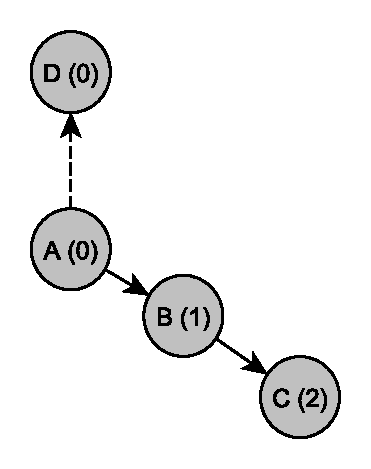
\includegraphics[width=0.3\textwidth]{Illustrations/BinarySearchTree.pdf}
\end{figure}

The nodes are drawn as circles, the keys indexing the nodes are in brackets after the tokens. The tokens A and D have the same key since they are in different trees (just linked with the ``above''-relation and depicted with a dotted arrow). Tokens A and B have no left children, therefore no nodes to the left. \\
The data structure \textbf{BinarySearchTree} implements a binary search tree as described. \\

The \textbf{BinarySearchTreeTrivial} data structure differs only in the insert-procedure from the normal BinarySearchTree data structure. Trees support intelligent procedures such as the rotation of leaves (to free up space), which BinarySearchTreeTrivial doesn't support. \footnote{This was rather a stage in development of the BinarySearchTree data structure than an individual idea. It worked well enough, which is why it was included in the tests.} \\

The \textbf{BinarySearchTreeLimitedDepth} data structure has a depth limit, i.e.\ inserts nodes only to a given depth of the tree. The depth of a tree describes the distance of the furthest child node to the root node of a tree. E.g.\ with depth limit 2, the exemplary problem file (see listing \ref{pf:example_pf}) would yield this representation:

\begin{figure}[H]
	\caption{BinarySearchTreeLimitedDepth representation}
	\label{img:binarysearchtreelimiteddepth_example_pf}
	\centering
	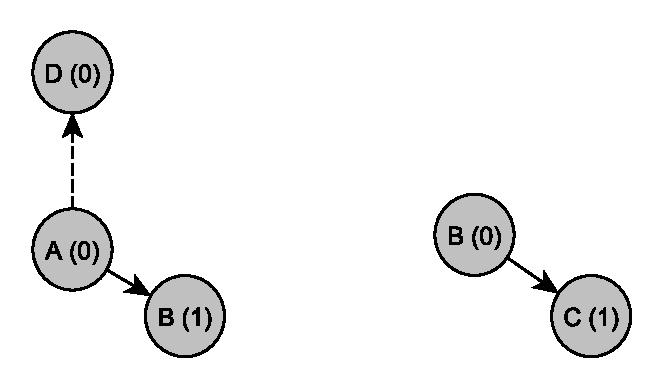
\includegraphics[width=0.6\textwidth]{Illustrations/BinarySearchTreeLimitedDepth.pdf}
\end{figure}

The token D can still be inserted into the first model since it doesn't increase the depth of either tree to a depth larger than 2. However, the second premise ``B left C'' will yield its own tree (with its own key numbering as well, so the token B has different keys in the two models). There is no alternative place to insert the token C into the first model: As token A's left child, it would be evaluated as being left of token B, which is incorrect. \\

The \textbf{BinarySearchTreeRandomTree} data structure builds a random binary search tree at each insert. Inserting tokens not by the order in which they ``arrived'' but randomly may even out the height of the tree. E.g. inserting keys 1, 2, 3, 4, 5, 6 in this order will yield a tree that is not very balanced. Inserting the same keys in a randomized order, e.g.\ as 3, 5, 1, 6, 2, 4 will yield a much more even tree.

\begin{figure}[H]
	\caption{Two binary search trees containing numbers from 1 to 6}
	\label{img:random_tree}
	\centering
	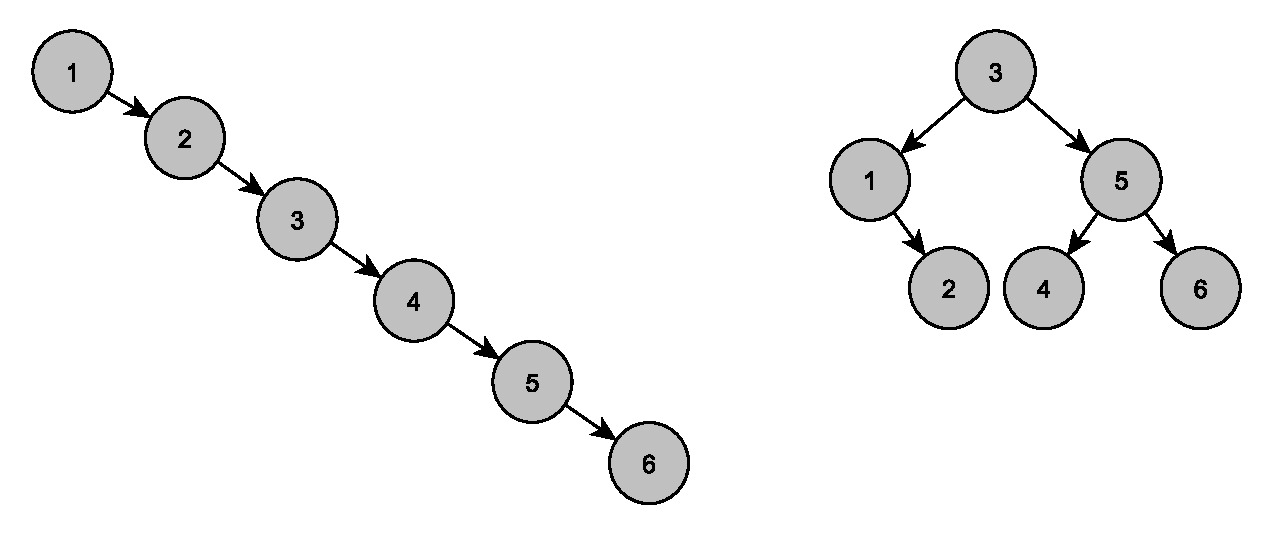
\includegraphics[width=0.9\textwidth]{Illustrations/BinarySearchTreeRandomTree.pdf}
\end{figure}

To this end, the BinarySearchTreeRandomTree has an InfiniteList data structure at its base. Into this structure, it inserts all the tokens from the premises. For every layer in the InfiniteList, it assigns a key linearly: The leftmost object receives key 1, the next key 2, etc. Then, choosing the items from the list randomly, it inserts the objects into a BinarySearchTree structure. \\
In this case, it would construct the same structure as InfiniteList (see listing \ref{inflist_example_pf}) and then assign key values. The assignment of key values is shown in table \ref{tab:random_search_tree_keys}.

\begin{table}[H]
\caption{Key assignment for random search tree} 
\label{tab:random_search_tree_keys}
\centering
	\begin{tabular}{c c}
	Token 	& Key value \\
	D		& 1 \\
	\hline
	A		& 1 \\
	B		& 2 \\
	C		& 3
	\end{tabular}
\end{table}

After first constructing a binary search tree just for token D for the first layer, it would construct a new binary search tree for the second layer and insert tokens A, B and C in a random order, then linking nodes A and D as described above to enable ``above''- and ``below''-relationships.

\subsubsection{Graph}
A graph stores information visually. A graph for the exemplary problem file (see listing \ref{pf:example_pf}) might look like this:

\begin{figure}[H]
	\caption{Graph representation}
	\label{img:graph_example_pf}
	\centering
	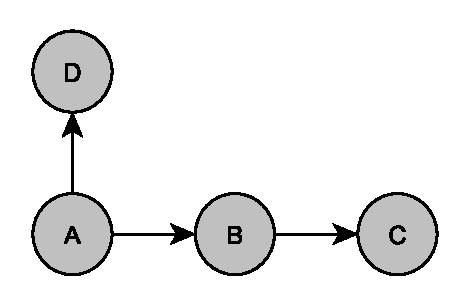
\includegraphics[width=0.4\textwidth]{Illustrations/Graph.pdf}
\end{figure}

Other forms could be imagined, e.g.\ without arrows indicating the relationship between tokens, or a representation that isn't based on a grid-like structure. DaStruct doesn't allow for ambiguous relationship (as in a non grid-like structure, see section \ref{sec:Bremen} for a computational implementation for ambiguous relationships).\\

A \textbf{Graph} model with the information from the exemplary problem file (see listing \ref{pf:example_pf}) would have this internal representation: \\ \\

\begin{lstlisting}[caption=Graph representation, label=graph_example_pf, frame=single]
[['',  'A', 'B', 'C', 'D'],
 ['A', 'x', 'l', 'l', 'b'],
 ['B', 'r', 'x', 'l', 'x'],
 ['C', 'r', 'r', 'x', 'x'],
 ['D', 'a', 'x', 'x', 'x']]
\end{lstlisting}

This representation represents an adjacency matrix \footnote{An adjacency matrix represents a graph by indicating which nodes are adjacent to each other, i.e.\ linked by an edge. In DaStruct, additionally the type of relationship between nodes (tokens) is specified.}. The first row and the first column contain the tokens which are contained in the model. The cells between them contain their relation. If the relation between B and C should be generated or evaluated, the row beginning with token B and the column beginning with token C will be chosen. The cell at their intersection describes the relation between B and C: 'l', short for left. \\
All other relations are similarly abbreviated. An 'x' denotes no recorded relationship.

\subsubsection{LinkedList}
The \textbf{LinkedList} data structure was implemented analogously to \cite{Krumnack.2011}'s implementation of linked lists, see section \ref{sec:Krumnack} for a description. LinkedLists are lists similar to the InfiniteList implementation, however they only support access in one direction (left to right). A linked list is a list of LinkedListNodes.
A LinkedListNode structure contains a token and a pointer. If a node is to the left of another node, its pointer will point to that node. If it is the rightmost node, its pointer won't point to another node. \\

The ``outer list'' that LinkedListNodes are contained in is necessary to enable three-dimensional indexing. Nodes that come first in the list are above nodes that come later in the list. \\
The outer list of LinkedListNodes for the exemplary problem file (see listing \ref{pf:example_pf}) would look like this:

\begin{lstlisting}[caption=LinkedList representation, label=linkedlist_example_pf, frame=single]
['D', 'A']
\end{lstlisting}

\noindent Expanding the nodes, it would look like this:

\begin{lstlisting}[caption=Expanded LinkedList representation, label=exp_linkedlist_example_pf, frame=single]
['D', 'A' -> 'B' -> 'C']
\end{lstlisting}

The arrows denote a pointer from one node to another.

\subsection{Data Methods and Additional Features}\label{sec:data_methods}
All data structures can freely be combined with different methods for treating the tokens and premises. Methods can describe different strategies for certain operations (such as inserts or merges), limit the size of a data structure or the memory strength of DaStruct.

\subsubsection{Insert strategy}
A type 2 premise, i.e. one where one token is known and present in at least one model and the other token is unknown, needs an insert procedure. In the exemplary problem file (see listing \ref{pf:example_pf}) the first premise ``A left B'' builds a model ``A, B'', the second premise ``B left C'' now requires an insert of token C into the previously constructed model ``A, B''. In this case the insert is deterministic and yields the model ''A, B, C''. However, for indeterminate inserts a strategy needs to be chosen. DaStruct supports the ff- and fff-strategy for inserts. For an explanation of these inserts, see section \ref{sec:determinacy}.

\subsubsection{Merge strategy}\label{sec:merge_strategy}
A type 4 premise, i.e. one where both tokens are known, but part of different models, requires a merge of these models. DaStruct supports two merge strategies: \\

\textbf{Integrate merge} \\
The integrate merge integrates two models into one model. Both single models will be deleted and a new model containing the merged information will be inserted into memory. \\

\textbf{Supermodel merge} \\
The supermodel merge will create supermodels instead of integrating models into one. This problem file:

\begin{lstlisting}[caption=Problem files for merges, label=pf_merging, frame=single]
P: A left B
P: C left D
P: E left F
P: B left C
P: D left E
\end{lstlisting}

would yield this hierarchy of supermodels:

\begin{figure}[H]
	\caption{Supermodel merge}
	\label{img:supermodel_merge}
	\centering
	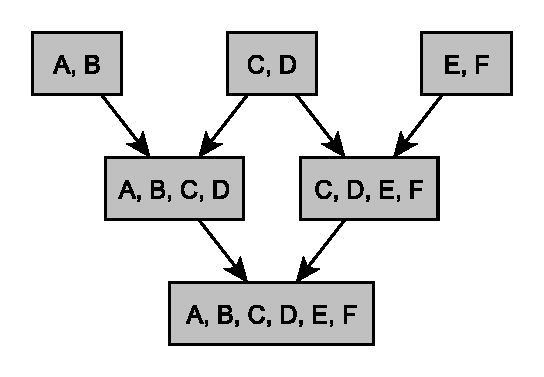
\includegraphics[width=0.6\textwidth]{Illustrations/supermodel_merge.pdf}
\end{figure}

The models on top are the models that represent the premises 1-3. Premises 4 and 5 specify the required merge operations. When performing the merges, the three models on top combine to the two supermodels on the second layer of the image. These two supermodels can again be combined to the supermodel of supermodels on the third layer of the image. \\
DaStruct has the option to limit the depth to which supermodels will be created. If that limit was set to 1 for the example above, the first layer of supermodels would still be constructed, the one below wouldn't. The premise ``A left F'' would then be evaluated as false. If the limit was set to 2, the second layer of supermodels would be constructed and the premise ``A left F'' would be evaluated as true.

\subsubsection{Distance on the neighborhood graph}
When premises call for indeterminate inserts, several models are possible representations of those premises. See section \ref{section:alternative_mental_models} for an explanation for how and when alternative mental models may be constructed. DaStruct has an optional limit for the distance on the neighborhood graph that an alternative model may have to the preferred mental model.

\subsubsection{Activation function}\label{sec:activation_function}
In neural networks \footnote{Computer systems inspired by the structure of biological neural networks, e.g.\ constructed similarly to the human visual system.}, activation functions serve as an analogue to the rate of action potential of a cell, i.e. the ``likelihood of a neuron firing''. In DaStruct, the activation function describes the process of forgetting information. \\
In 1885, Hermann Ebbinghaus started testing his own memory: He memorized sheets of nonsense syllables and tested his remaining knowledge at certain points in time \citep{Ebbinghaus.1913}. The resulting \textit{forgetting curve} describes how many of these syllables he could still remember at a given point in time. Extrapolating his data, the function
\begin{gather}
R = e^{(-t/S)}
\end{gather}
is an approximation of his forgetting curve. $R$ is the amount of information that was retained, $t$ is the point in time after the learning of the information and $S$ is a factor that describes the ``memory strength''. Increasing it will increase the amount of information that is remembered at a given point in time. \\

This curve is the basis for some activation functions that were used in experiments with DaStruct. The forgetting of tokens was modeled, not the forgetting of relations between tokens. Tokens are somewhat similar to Ebbinghaus' syllables since in the experiment they had names such as A, B or C and were therefore presumably not considerably more meaningful to participants than Ebbinghaus' random syllables. Ebbinghaus' curve describes the process of forgetting a set of syllables and therefore one chunk of information. For DaStruct, it was interesting to model the forgetting of several tokens. \\

\cite*{Yffelti.2016} proposes a function that works on the basis of Ebbinghaus' forgetting curve when several pieces of information are added into a memory system. In DaStruct's case, the time points of insertion of a token into memory were set as the premise number \footnote{The first premise in a problem has premise number 1, the second has premise number 2 and so on.} in which a token was first seen. It is assumed that every token has the same strength of insertion, so no token is inserted more strongly than other tokens. In that case, \cite{Yffelti.2016} proposes the following formula based on the superposition principle\footnote{\url{https://en.wikipedia.org/wiki/Superposition_principle}}:
\begin{gather}
I(t) = \Delta I \cdot \sum \limits_{i=1}^n  e^{-\frac{t-i \cdot \Delta t}{S}} \cdot \theta(t - t_i),
\end{gather}
where 
\begin{equation}
  \theta(t)=\begin{cases}
               1, ~~t \geq 0, \\
               0, ~~t < 0
            \end{cases}
\end{equation}
is the Heaviside function \footnote{\url{https://en.wikipedia.org/wiki/Heaviside_step_function}}. \\

For different memory strength factors $S$, this function is shown plotted in figures \ref{fig:Equidistant equiintense information injections into a system with memory strength 1} and \ref{fig:Equidistant equiintense information injections into a system with memory strength 2}.

\begin{figure}[H]
\centering
\includegraphics[width=0.7\textwidth]{Illustrations/Equidistant_equiintense_with_S=1.png}
\caption{Equidistant information injections with equal intensities ($\Delta I_i = 1$) into a system with memory strength $S=1$.}
\label{fig:Equidistant equiintense information injections into a system with memory strength 1}
\end{figure}

\begin{figure}[H]
\centering
\includegraphics[width=0.7\textwidth]{Illustrations/Equidistant_equiintense_with_S=2.png}
\caption{Equidistant information injections with equal intensities ($\Delta I_i = 1$) into a system with memory strength $S=2$.}
\label{fig:Equidistant equiintense information injections into a system with memory strength 2}
\end{figure}

When using \cite{Yffelti.2016}'s model, two assumptions must be borne in mind:
\begin{itemize}
	\item \cite{Yffelti.2016}'s result is obtained for continuous time, whereas DaStruct is interested in discrete consequent time moments, so that the time continuum is quasi projected into a series of discrete points,
	\item the length of the series is actually limited, i.e., while the theoretical limit of $I(t)$ in  \cite{Yffelti.2016}'s model is $\infty$, we only consider the function on a limited interval.
\end{itemize}

For DaStruct, I used the upper values of this function with memory strengths 2 and 3 to obtain a limit that denotes which tokens are forgotten again, assuming that tokens that were seen the longest ago are forgotten first. This may seem low when considering \cite{Miller.1956}'s magical number of 7 (as a limit of how many slots the human working memory approximately has for chunks of information). However, two tokens in memory may mean more than two slots concurrently filled. Two tokens additionally mean one relationship between them. Three tokens already mean three tokens and two or even three relationships. It is to be assumed that these relationships are encoded in a cognitively efficient way (which is what the model theory describes). Still, the relationships do need some encoding and will fill some part of human working memory. \\

In practice, with this problem file:

\begin{lstlisting}[caption=Problem file, frame=single]
P: A left B
P: B left C
P: D above A
\end{lstlisting}

This is the table denoting the time step at which each token was first seen:

\begin{table}[H]
	\begin{tabular}{| c c |}
	\hline
	Time step 	& Token \\
	1			& A		\\
	1			& B		\\
	2			& C		\\
	3			& D		\\
	\hline
	\end{tabular}
	\caption{At which time step tokens were first seen}
\end{table}

Tokens A and B were both seen in the first premise and thereby time step 1. The function given by \cite{Yffelti.2016} yields the following results for each time step:

\begin{table}[H]
	\begin{tabular}{| c c |}
	\hline
	Time step 	& Result of \cite{Yffelti.2016}'s function with memory strength $S$ = 2	\\
	1			& 1											\\
	2			& 1.6065									\\
	3			& 1.9646									\\
	\hline
	\end{tabular}
	\caption{Result of \cite{Yffelti.2016}'s function with memory strength $S$ = 2 for three time steps}
\end{table}

Using \cite{Yffelti.2016}'s forgetting curve model, we would have 1.96 information units remaining at time step 3. That is, at this point in time, $3 - 1.96 = 1.04 \approx 1$ information units are forgotten. Which ones are forgotten? Naturally, the first one, since it has been seen the longest ago. This would mean that tokens A and B are not accessible anymore. The premise ``B left C'' would now be categorized as a type 1/type 3 premise instead of a type 2 premise.

\subsection{Difficulty Measures and Cumulated Difficulty Measures}\label{sec:difficulty_measures}
While processing the premises and conclusion, DaStruct collects a variety of difficulty measures. PRISM already collects some difficulty measures (see \ref{sec:PRISM} for a description of these). DaStruct aims to obtain a higher resolution of measures. \\
The difficulty measures that were collected were chosen 
\begin{itemize}
	\item for the fact that they were easily implementable, e.g.\ if implementing them followed naturally out of their computational implementation,
	\item for the fact that a similar (or the same) difficulty measure was implemented in PRISM,
	\item for the fact that the author assumed that they would measure difficulty.
\end{itemize}
This exemplary problem set will help illustrate the difficulty measures collected by DaStruct:

\begin{lstlisting}[caption=Exemplary problem file, label=pf:example_pf_diff_measures, frame=single]
P: A left B
P: B left C
P: E right D
P: D right C
\end{lstlisting}

\noindent The explanations of difficulty measures are based on an unlimited data structure. The results of the measures will vary for limited data structures.

\subsubsection{Collected difficulty measures}
The following single difficulty measures were collected by DaStruct:

\begin{itemize}
	\item \textbf{Focus move operations}: Measures whether the focus was moved at all. The focus is 		analogous to PRISM's head movements (see section \ref{sec:PRISM} for those). The focus is always 		moved to the last token that was important. When considering the exemplary problem file (see listing \ref{pf:example_pf_diff_measures}), for the first premise one focus move operation would be performed. First, the token A would be inserted into the model and the focus would be on token A. Immediately thereafter, token B would be inserted and focus would be shifted to it. For premise 2, the focus would be shifted from token B to token C. In premise 3, the focus is shifted from token E to token D, for premise 4 no focus move operation is necessary since in both the models that are merged the focus lies on the tokens that describe the merge operation.\\
	Altogether, the exemplary problem file has 3 focus move operations.
	\item \textbf{Focus move distance}: Measures how far the focus was moved. In the exemplary problem file (see listing \ref{pf:example_pf_diff_measures}), every focus move operation only moves the focus a distance of 1. If the distance between tokens is bigger, the focus move distance increases. E.g.\ given the premises ``A left B'', ``B left C'' and ``D left A'', the focus would have to move from token C to token A for the third premise. The move distance of that move operation would be 2.\\
	Altogether, the exemplary problem file has a focus move distance of 3.
	\item \textbf{Focus key distance}: Measures the key distance when performing a focus move operation in a BinarySearchTree. When the node in focus changes in a BinarySearchTree, this measure collects the key distance between them. \\
	Altogether, the exemplary problem file has a focus key distance of 3, when utilizing the base data structure BinarySearchTree.
	\item \textbf{Write operations}: Measures the amount of write operations. When no merge operations are required, this equates to the number of tokens that are mentioned. If a merge operation is required and the merge strategy is set to integrate, one set of tokens need to be ``rewritten'', i.e.\ integrated into another model. This increases the write operation measure to a number higher than the number of tokens mentioned. In the exemplary problem file (see listing \ref{pf:example_pf_diff_measures}), the model ``D, E'' needs to be inserted into the model ``A, B, C'' on the basis of the premise ``D right C''. 5 write operations were performed up to this point. If the merge strategy is set to integrate, the model ``D, E'' would need to be rewritten, thus creating the merged model ``A, B, C, D, E''.\\
	Altogether, the exemplary problem file requires 7 write operations if the merge strategy is set to integrate and 5 if the merge strategy is set to supermodel.
	\item \textbf{Insert operations}: Measures the amount of insert operations. For a type 2 premise, a token needs to be inserted into an existing model. \\
	Altogether, the exemplary problem file requires one insert operation. The first and third premise are type 1/type 3 premises and do not specify an insert. The fourth premise is a type 4 premise. Only the second premise is a type 2 premise and requires one insert operation.
	\item \textbf{Merge operations}: Measures the amount of merge operations. For a type 4 premise, two models need to be merged. \\
	Altogether, the exemplary problem file requires one merge operation, as specified in the fourth premise.
	\item \textbf{Supermodels created}: Measures the amount of supermodels that were created. If a merge is performed, this increases the amount of supermodels. For the example in \ref{sec:merge_strategy}, this would be 3. \\
	Altogether, the exemplary problem file would, if executed with the supermodel merge strategy, require one supermodel to be created.
	\item \textbf{Supermodels accessed}: Measures the amount of supermodels that needed to be accessed. If a conclusion is to be evaluated, supermodels are checked going iteratively higher up the hierarchy of supermodels. How many supermodels needed to be checked to verify a conclusion is what is measured here. If a conclusion is inconsistent, all supermodels are accessed. \\
	Altogether, the exemplary problem file requires no supermodels to be accessed, since it contains no conclusion.
	\item \textbf{Grouping operations}: Measures the amount of times the content of a model is grouped for a merge operation. In preparation for a merge operation, the entire content of both models is grouped. \\
	Altogether, the exemplary problem file requires one grouping operation.
	\item \textbf{Grouping size}: Measures the size (in amount of tokens) that were grouped for a merge. In the case of the exemplary problem file (see listing \ref{pf:example_pf_diff_measures}), the second model is merged into the first model. Both models are grouped. They contain five tokens. \\
	Altogether, the exemplary problem file requires a grouping of size 5.
	\item \textbf{Premise direction changes}: Measures how often the relationship changes that is specified in the premises. In the exemplary problem file (see listing \ref{pf:example_pf_diff_measures}), the first two premises contain the relationship ``left'', while the second two premises contain the relationship ``right''. This change is measured. \\
	Altogether, the exemplary problem file has one premise direction change.
	\item \textbf{Focus direction change}: Measures how often the direction of the focus changed. Every time a focus move operation occurs, the focus moves into a direction. E.g.\ in the first premise of the exemplary problem file (see listing \ref{pf:example_pf_diff_measures}), the focus moves from token A to token B. Since token A is to the left of token B, the focus moves into the direction right. That direction stays the same for premise two. In premise three, no change of focus direction occurs, since ``E right D'' is the initial premise for a new model. Since premise four does not require any focus move operation, there's no focus direction change required. \\
	Altogether, the exemplary problem file has no focus direction changes.
	\item \textbf{Linked List followed a pointer}: Measures how often a pointer was followed in a LinkedList data structure (see section \ref{sec:data_methods} for an explanation of pointers). \\
	Altogether, the exemplary problem file requires 20 pointers to be followed.
	\item \textbf{Model attention changes}: Measures how often the attention changes from one model to another. In the exemplary problem file (see listing \ref{pf:example_pf_diff_measures}), the first two premises describe one model. The third premise instantiates a new model which the attention is shifted to. The fourth premise describes a merge. The attention is shifted to the newly created merged model. \\
	Altogether, the exemplary problem file requires 2 model attention changes.
	\item \textbf{Annotation operations}: Measured how often ambiguous tokens were inserted. Every time a token is inserted whose position is described by an indeterminate premise, this ambiguity is noted inside the model. If a model variation phase is enabled (see section \ref{section:alternative_mental_models}), these annotations enable the correct local transformation to the next node on the neighborhood graph. \\
	Altogether, the exemplary problem file requires no annotation operations.
	\item \textbf{Model counter}: Measures how many single models were created. In the exemplary problem file (see listing \ref{pf:example_pf_diff_measures}), two models are instantiated, once in premise 1 and once in premise 3. They are both type 1/type 3 premises and therefore instantiate a new model. \\
	Altogether, the exemplary problem file has a model count of 2.
	\item \textbf{Deletion of models}: Measures how often models are deleted. In the exemplary problem file (see listing \ref{pf:example_pf_diff_measures}), two models are instantiated, once in premise 1 and once in premise 3. They are merged by premise 4. \\
	Altogether, the exemplary problem file requires one deletion of models.
	\item \textbf{Amount of relationships in Graph}: Measures the amount of relationships recorded in a model of data structure type Graph (divided by two, in order not to count relationships twice). \\
	Altogether, the amount of relationships for the exemplary problem file when using data structure type Graph was 20/2 = 10.
	\item \textbf{BinarySearchTree Depth}: Measures the maximum depth of BinarySearchTree models. For all models, this measures the BinarySearchTree with the highest depth. \\
	Altogether, the maximum depth for the exemplary problem file when using data structure type BinarySearchTree was 4.
\end{itemize}

\subsubsection{Summed up difficulty measures}\label{sec:diff_measures_summed_up}
To simplify testing DaStruct, the following sums of difficulty measures were used:
``Sum of difficulty measures'', ``Sum of focus operations'', ``Sum of focus operations (focus distance not considered)'', ``Sum of focus operations (only focus distance considered)'', ``Sum of merge operations'', ``Sum of model operations''.
\begin{itemize}
	\item \textbf{Sum of difficulty measures}: The sum of all difficulty measures that were collected
	\item \textbf{Sum of focus operations}: The sum of all focus operations. These are:
	\begin{itemize}
		\item Focus move operations
		\item Focus move distance
		\item Focus direction changes
		\item Model in attention changes
	\end{itemize}
	\item \textbf{Sum of focus operations (focus distance not considered)}: Sum of focus operations, but without Focus move distance
	\item \textbf{Sum of focus operations (focus move operations not considered)}: Sum of focus operations, but without Focus move operations. \\
	The two sums of focus operations were differentiated to see whether focus move operations or focus move distance had the bigger effect
	\item \textbf{Sum of merge operations}: The sum of all merge operations. These are:
	\begin{itemize}
		\item Merge operations
		\item Supermodels created
		\item Supermodels accessed
		\item Grouping operations
		\item Grouping size
	\end{itemize}
	\item \textbf{Sum of model operations}: The sum of all model operations. These are:
	\begin{itemize}
		\item Supermodels created
		\item Model in attention changes
		\item Model counter
		\item Deletion of models
	\end{itemize}
\end{itemize}

\section{Experiments with DaStruct}
Two experiments were designed comparing DaStruct's performance with the performance of human test participants. \\

The data that was used was collected in January 2012 in an online experiment (named Comparison1). 40 test subjects participated in the experiment (mean  age 34.97, standard deviation of age 10.28, 57.5\% female).
These 40 participants did the first part of the experiment: 16 problems were shown, each consisting of two premises and one conclusion. Of those 16 problems, 8 were consistent and 8 were inconsistent. \\
Of the 40 participants, 35 also completed the second part of the experiment (mean age 33.94, standard deviation age 9.73, 50\% female). 48 problems were shown, each consisting of three premises and one conclusion. Of those 48 problems, 24 were consistent and 24 were inconsistent. \\
Participants could read the premises in a self-paced way. When they finished reading one premise and the next premise appeared, the last premise disappeared. Their reading time for the premises and answer time for the conclusion was measured. \\

Using this data, two experiments were designed. The first experiment tried to predict the difficulty of a problem set. The questions motivating this experiment were: Is it possible to predict the difficulty that a problem set has for human participants? I.e., does a growing difficulty measure indicate that less participants are able to solve a problem correctly? If so, which difficulty measures are the best predictors? Section \ref{sec:exp1} describes this experiment. Results were somewhat inconclusive. \\
The second experiment tried to match each participant to a specific combination of data structure and data methods. The question motivating this experiment was: Is it possible to say for an individual test participant which data structure or data method models their reasoning process best? Section \ref{sec:exp2} describes this experiment. It was apparent that from all of DaStruct's data structures, BinarySearchTree or derivatives most closely matched participants' reasoning process. Often, the data structure could clearly be shown to be limited in depth. Participants could very clearly be matched to a data structure, the limit of that data structure, an insert strategy, an activation function and whether or not they performed merge operations.

\subsection{Predicting Difficulty of a Problem Set}\label{sec:exp1}
In a first experiment, the following question was to be tested: Is it possible to predict mean human ability to solve a problem by the difficulty measures that DaStruct produces? \\
In other words: Do difficulty measures correlate with the percentage of test subjects who solved a problem correctly?

\subsubsection{The Experiment}
In a first analysis, the first set of problems which contained two premises and a conclusion and the second set of problems containing three premises and a conclusion were evaluated separately. In a second analysis, all problems were evaluated together. The following tables show how many problems could be solved correctly by a given data structure as well as the correlation coefficients \footnote{Computed using Pearson product-moment correlation coefficient} between difficulty measures generated by DaStruct and the percentage of test subjects able to correctly solve a problem. The correlation coefficient should be negative, since a higher difficulty measure should correlate with fewer participants solving the problem correctly and vice versa. \\
In those problems with only two premises and one conclusion, no merges were required. Therefore, merge operations and model operations were not considered for these problems. \\
There was no activation function specified, i.e.\ tokens were remembered indefinitely. \\
In the following tables, the columns with the highest correlation factors were highlighted (and sometimes additionally cells from other columns with even higher correlation factors).\\
The rows in the tables are ``Number of correctly solved problem instances'', ``Sum of difficulty measures'', ``Sum of focus operations'', ``Sum of focus operations (focus distance not considered)'', ``Sum of focus operations (only focus distance considered)'', ``Sum of merge operations'', ``Sum of model operations''. To save space, in the tables these row names were shortened. See section \ref{sec:diff_measures_summed_up} for a description of these difficulty measures. Column names correspond to data structures. PRISM is \cite{Ragni.2013}'s computational implementation, see section \ref{sec:PRISM} for a description. All other data structures are from DaStruct, see section \ref{sec:data_structs} for descriptions. Numbers after data structure names denote the limit for size that was applied.

\begin{table}[H]
	\hspace*{-1.5cm}
	\begin{tabular}{ p{2cm}  c  g  c  g  c  c  c  c  c  c  c }
	& \rot{PRISM} & \rot{InfiniteList} & \rot{BoundedList2} & \rot{BoundedList3} & \rot{BinarySearchTree} & \rot{BSTRandomTree} & \rot{BSTLimitedDepth2} & \rot{BSTLimitedDepth3} & \rot{BSTTrivial} & \rot{Graph} &	\rot{LinkedList} \\
	Solved instances & 16 & 16 & 8 & 16 & 16 & 15 & 4 & 4 & 16 & 16 & 16\\
	Difficulty & -0.382 & -0.382 & \cellcolor{lightgray}-0.49 & -0.382 & -0.2 & -0.22 & -0.483 & -0.483 & -0.302 & 0.356 & -0.192\\
	Focus & & -0.239 & & -0.239 & -0.129 & -0.21 & -0.431 & -0.431 & -0.199 & 0.493 & -0.09 \\
	(no $\delta$) & & -0.239 & & -0.239 & -0.189 & -0.23 & -0.25 & -0.25 & -0.194 & 0.507 & -0.129\\
	(only $\delta$) & & -0.239 & & -0.239 & -0.09 & -0.2 & -0.441 & -0.441 & -0.199 & 0.47 & -0.085\\
	\end{tabular}
	\hspace*{-1.5cm}
	\caption{Comparison1 - Two premises and one conclusion, solved using ff-strategy}
	\label{tab:3prem-ff}
	
	\vspace{1cm}
	
	\hspace*{-1.5cm}
	\begin{tabular}{ p{2cm}  c  c  c  c  c  c  g  g  c  c  c }
	& \rot{PRISM} & \rot{InfiniteList} & \rot{BoundedList2} & \rot{BoundedList3} & \rot{BinarySearchTree} & \rot{BSTRandomTree} & \rot{BSTLimitedDepth2} & \rot{BSTLimitedDepth3} & \rot{BSTTrivial} & \rot{Graph} &	\rot{LinkedList} \\
	Solved instances & 16 & 16 & 8 & 16 & 16 & 16 & 8 & 8 & 16 & 16 & 16\\
	Difficulty & -0.239 & -0.382 & \cellcolor{lightgray}-0.49 & -0.382 & -0.15 & -0.03 & -0.2 & -0.2 & -0.167 & 0.356 & -0.192\\
	Focus & & -0.239 & & -0.239 & -0.129 & -0.14 & -0.204 & -0.204 & -0.199 & 0.493 & -0.09 \\
	(no $\delta$) & & -0.239 & & -0.239 & -0.189 & -0.013 & -0.121 & -0.121 & -0.194 & 0.507 & -0.129\\
	(only $\delta$) & & -0.239 & & -0.239 & -0.09 & -0.12 & -0.173 & -0.173 & -0.199 & 0.47 & -0.085\\
	\end{tabular}
	\hspace*{-1.5cm}
	\caption{Comparison1 - Two premises and one conclusion, solved using fff-strategy}
	\label{tab:3prem-fff}
\end{table}

\begin{table}[H]
	\hspace*{-1.5cm}
	\begin{tabular}{ p{2cm}  c  g  g  c  c  c  c  c  c  c  c }
	& \rot{PRISM} & \rot{InfiniteList} & \rot{BoundedList2} & \rot{BoundedList3} & \rot{BinarySearchTree} & \rot{BSTRandomTree} & \rot{BSTLimitedDepth2} & \rot{BSTLimitedDepth3} & \rot{BSTTrivial} & \rot{Graph} &	\rot{LinkedList} \\
	Solved instances 	& 48 		& 48 		& 25 		& 25 		& 45 	& 48 		& 20 									& 18 		& 45 		& 48 		& 48\\
	Difficulty 			& -0.345 	& -0.307 	& -0.279 	& -0.229 	& 0.146 & -0.115 	& -0.021 								& 0.087 	& 0.136 	& 0.013 	& 0.005\\
	Focus 				& 			& -0.198 	& -0.316 	& -0.152 	& 0.173 & -0.069 	& 0.087 								& 0.124 	& 0.176 	& 0.274 	& -0.026\\
	(no $\delta$) 		& 			& -0.279 	& -0.348 	& -0.186 	& 0.009 & -0.301 	& 0.116 								& 0.114 	& -0.283 	& -0.333	& -0.02\\
	(only $\delta$) 	& 			& -0.285 	& -0.348 	& -0.186 	& 0.173 & -0.087 	& 0.09 									& 0.112 	& 0.188 	& 0.282 	& -0.02\\
	Merge 				& 			& -0.251 	& -0.251 	& -0.251 	& -0.251& -0.251 	& -0.251 								& -0.251 	& -0.251 	& -0.251 	& -0.251\\
	Model 				& 			& -0.276 	& -0.379 	& -0.282 	& -0.271& -0.271 	& -0.185 								& -0.271 	& -0.271 	& -0.276 	& -0.276\\
	\end{tabular}
	\hspace*{-1.5cm}
	\caption{Comparison1 - Three premises and one conclusion, solved using ff-strategy and integrate-merge}
	\label{tab:4prem-ff-integrate}
	
	\vspace{1cm}
	
	\hspace*{-1.5cm}
	\begin{tabular}{ p{2cm}  c  g  g  g  c  c  c  c  c  c  c }
	& \rot{PRISM} & \rot{InfiniteList} & \rot{BoundedList2} & \rot{BoundedList3} & \rot{BinarySearchTree} & \rot{BSTRandomTree} & \rot{BSTLimitedDepth2} & \rot{BSTLimitedDepth3} & \rot{BSTTrivial} & \rot{Graph} &	\rot{LinkedList} \\
	Solved instances 	& 48 		& 48 		& 25 		& 25 		& 48 	& 48 		& 14 									& 27		& 48 		& 48 		& 48\\
	Difficulty 			& -0.345 	& -0.307 	& -0.279 	& -0.279 	& 0.148 & -0.053 	& 0.029 								& 0.217 	& 0.147 	& 0.013 	& 0.005\\
	Focus 				&  			& -0.198 	& -0.316 	& -0.316 	& 0.162 & -0.014 	& 0.125 								& 0.213 	& 0.167 	& 0.274 	& -0.026\\
	(no $\delta$) 		& 			& -0.279 	& -0.348 	& -0.349 	& 0.073 & -0.243 	& 0.095 								& 0.078 	& -0.259 	& 0.133 	& -0.333\\
	(only $\delta$) 	& 			& -0.285 	& -0.348 	& -0.349 	& 0.16 	& -0.03 	& 0.128 								& 0.22 		& 0.179 	& 0.282 	& -0.02\\
	Merge 				& 			& -0.251 	& -0.251 	& -0.251 	& -0.251& -0.251 	& -0.251 								& -0.251 	& -0.251 	& -0.251 	& -0.251\\
	Model 				& 			& -0.276 	& -0.379 	& -0.379 	& -0.271& -0.271 	& -0.196 								& -0.271 	& -0.271 	& -0.276 	& -0.276\\
	\end{tabular}
	\hspace*{-1.5cm}
	\caption{Comparison1 - Three premises and one conclusion, solved using fff-strategy and integrate-merge}
	\label{tab:4prem-fff-integrate}
\end{table}
	
\begin{table}[H]
	\hspace*{-1.5cm}
	\begin{tabular}{ p{2cm}  c  c  g  c  c  c  c  c  c  c  c }
	& \rot{PRISM} & \rot{InfiniteList} & \rot{BoundedList2} & \rot{BoundedList3} & \rot{BinarySearchTree} & \rot{BSTRandomTree} & \rot{BSTLimitedDepth2} & \rot{BSTLimitedDepth3} & \rot{BSTTrivial} & \rot{Graph} &	\rot{LinkedList} \\
	Solved instances 	& 48		& 41		& 25		& 25		& 38		& 41		& 16								& 11		& 38		& 41		& 41\\
	Difficulty 			& -0.345	& -0.278	& -0.3		& -0.194	& -0.045	& -0.06		& 0.155								& 0.274		& -0.08		& 0.14		& -0.122\\
	Focus 				& 			& -0.021	& -0.379	& 0.044		& -0.036	& -0.027	& 0.16								& 0.294		& -0.085	& 0.149		& -0.006\\
	(no $\delta$) 		& 			& -0.139	& -0.425	& -0.056	& -0.005	& 0.05		& 0.152								& 0.346		& -0.066	& 0.148		& 0.056\\
	(only $\delta$) 	& 			& -0.144	& -0.425	& -0.056	& -0.045	& -0.035	& 0.162								& 0.294		& -0.079	& 0.148		& -0.038\\
	Merge 				& 			& -0.251	& -0.251	& -0.251	& -0.251	& -0.251	& -0.251							& -0.251	& -0.251	& -0.251	& -0.251\\
	Model 				& 			& -0.282	& -0.425	& -0.291	& -0.282	& -0.282	& -0.234							& -0.282	& -0.282	& -0.282	& -0.282\\
	\end{tabular}
	\hspace*{-1.5cm}
	\caption{Comparison1 - Three premises and one conclusion, solved using ff-strategy and supermodel-merge with 0 supermodels admitted}
	\label{tab:4prem-ff-supermodel0}
	
	\vspace{1cm}
	
	\hspace*{-1.5cm}
	\begin{tabular}{ p{2cm}  c  c  g  c  c  c  c  c  c  c  c }
	& \rot{PRISM} & \rot{InfiniteList} & \rot{BoundedList2} & \rot{BoundedList3} & \rot{BinarySearchTree} & \rot{BSTRandomTree} & \rot{BSTLimitedDepth2} & \rot{BSTLimitedDepth3} & \rot{BSTTrivial} & \rot{Graph} &	\rot{LinkedList} \\
	Solved instances 	& 48		& 48		& 32		& 32		& 45		& 48		& 23								& 18		& 45		& 41		& 48\\
	Difficulty 			& -0.345	& -0.393	& -0.347	& -0.312	& -0.074	& -0.222	& 0.107								& 0.244		& -0.11		& 0.102		& -0.288\\
	Focus 				& 			& -0.198	& -0.316	& -0.152	& -0.036	& -0.192	& 0.159								& 0.294		& -0.085	& 0.149		& -0.187\\
	(no $\delta$) 		& 			& -0.279	& -0.348	& -0.186	& -0.005	& -0.14		& 0.152								& 0.346		& -0.066	& 0.148		& -0.133\\
	(only $\delta$) 	& 			& -0.285	& -0.348	& -0.186	& -0.045	& -0.194	& 0.162								& 0.295		& -0.079	& 0.148		& -0.21\\
	Merge 				& 			& -0.345	& -0.345	& -0.345	& -0.251	& -0.251	& -0.345							& -0.345	& -0.251	& -0.251	& -0.251\\
	Model 				& 			& -0.276	& -0.379	& -0.282	& -0.276	& -0.276	& -0.24								& -0.276	& -0.276	& -0.276	& -0.276\\
	\end{tabular}
	\hspace*{-1.5cm}
	\caption{Comparison1 - Three premises and one conclusion, solved using ff-strategy and supermodel-merge with 1 supermodel admitted}
	\label{tab:4prem-ff-supermodel1}
\end{table}	
	
\begin{table}[H]
	\hspace*{-1.5cm}
	\begin{tabular}{ p{2cm}  c  c  g  c  c  c  c  c  c  c  c }
	& \rot{PRISM} & \rot{InfiniteList} & \rot{BoundedList2} & \rot{BoundedList3} & \rot{BinarySearchTree} & \rot{BSTRandomTree} & \rot{BSTLimitedDepth2} & \rot{BSTLimitedDepth3} & \rot{BSTTrivial} & \rot{Graph} &	\rot{LinkedList} \\
	Solved instances 	& 48		& 41		& 25		& 25		& 41		& 41		& 10								& 20		& 41		& 41		& 41\\
	Difficulty 			& -0.345	& -0.278	& -0.3		& -0.194	& -0.052	& -0.044	& 0.133								& 0.2		& -0.075	& 0.14		& -0.122\\
	Focus 				& 			& -0.021	& -0.379	& 0.044		& -0.029	& 0.002		& 0.155								& 0.193		& -0.06		& 0.149		& -0.006\\
	(no $\delta$) 		& 			& -0.139	& -0.425	& -0.056	& 0.044		& 0.047		& 0.122								& 0.12		& -0.004	& 0.148		& 0.056\\
	(only $\delta$) 	& 			& -0.144	& -0.425	& -0.056	& -0.038	& -0.006	& 0.155								& 0.19		& -0.054	& 0.148		& -0.038\\
	Merge 				& 			& -0.251	& -0.251	& -0.251	& -0.251	& -0.251	& -0.251							& -0.251	& -0.251	& -0.251	& -0.251\\
	Model 				& 			& -0.282	& -0.425	& -0.291	& -0.282	& -0.282	& -0.249							& -0.282	& -0.282	& -0.282	& -0.282\\
	\end{tabular}
	\hspace*{-1.5cm}
	\caption{Comparison1 - Three premises and one conclusion, solved using fff-strategy and supermodel-merge with 0 supermodels admitted}
	\label{tab:4prem-fff-supermodel0}
	
	\vspace{1cm}
	
	\hspace*{-1.5cm}
	\begin{tabular}{ p{2cm}  c  c  g  c  c  c  c  c  c  c  c }
	& \rot{PRISM} & \rot{InfiniteList} & \rot{BoundedList2} & \rot{BoundedList3} & \rot{BinarySearchTree} & \rot{BSTRandomTree} & \rot{BSTLimitedDepth2} & \rot{BSTLimitedDepth3} & \rot{BSTTrivial} & \rot{Graph} &	\rot{LinkedList} \\
	Solved instances 	& 48		& 48		& 32		& 32		& 48		& 48		& 17								& 27		& 48		& 41		& 48\\
	Difficulty 			& -0.345	& -0.393	& -0.347	& -0.312	& -0.076	& -0.185	& 0.103								& 0.175		& -0.102	& 0.102		& -0.288\\
	Focus 				& 			& -0.198	& -0.316	& -0.152	& -0.029	& -0.099	& 0.155								& 0.193		& -0.06		& 0.149		& -0.187\\
	(no $\delta$) 		& 			& -0.279	& -0.348	& -0.186	& 0.044		& -0.156	& 0.122								& 0.12		& -0.004	& 0.148		& -0.133\\
	(only $\delta$) 	& 			& -0.285	& -0.348	& -0.186	& -0.038	& -0.101	& 0.155								& 0.19		& -0.054	& 0.148		& -0.21\\
	Merge 				& 			& -0.345	& -0.345	& -0.345	& -0.251	& -0.251	& -0.345							& -0.345	& -0.251	& -0.251	& -0.251\\
	Model 				& 			& -0.276	& -0.379	& -0.282	& -0.276	& -0.276	& -0.251							& -0.276	& -0.276	& -0.276	& -0.276\\
	\end{tabular}
	\hspace*{-1.5cm}
	\caption{Comparison1 - Three premises and one conclusion, solved using fff-strategy and supermodel-merge with 1 supermodel admitted}
	\label{tab:4prem-fff-supermodel1}
\end{table}

\begin{table}[H]
	\hspace*{-1.5cm}
	\begin{tabular}{ p{2cm}  c  g  g  c  c  c  c  c  c  c  c }
	& \rot{PRISM} & \rot{InfiniteList} & \rot{BoundedList2} & \rot{BoundedList3} & \rot{BinarySearchTree} & \rot{BSTRandomTree} & \rot{BSTLimitedDepth2} & \rot{BSTLimitedDepth3} & \rot{BSTTrivial} & \rot{Graph} &	\rot{LinkedList} \\
	Solved instances 	& 64		& 64		& 33		& 41		& 61		& 64		& 24								& 22		& 61		& 64		& 64\\
	Difficulty 			& -0.524	& -0.517	& -0.445	& -0.409	& 0.026		& -0.373	& -0.06								& -0.139	& 0.012		& -0.413	& -0.281\\
	Focus 				& 			& -0.444	& -0.477	& -0.329	& 0.125		& -0.333	& 0.103								& 0.026		& 0.167		& 0.013		& -0.279\\
	(no $\delta$) 		& 			& -0.483	& -0.522	& -0.378	& -0.09		& -0.49		& 0.055								& -0.05		& -0.355	& -0.116	& -0.478\\
	(only $\delta$) 	& 			& -0.49		& -0.522	& -0.378	& 0.157		& -0.318	& 0.13								& 0.044		& 0.193		& 0.005		& -0.26\\
	Merge 				& 			& -0.356	& -0.356	& -0.356	& -0.356	& -0.356	& -0.356							& -0.356	& -0.356	& -0.356	& -0.356\\
	Model 				& 			& -0.375	& -0.554	& -0.45		& -0.372	& -0.372	& -0.336							& -0.372	& -0.372	& -0.375	& -0.375\\
	\end{tabular}
	\hspace*{-1.5cm}
	\caption{Comparison1, solved using ff-strategy and integrate-merge}
	\label{tab:all-comp1-ff-integrate}
	
	\vspace{1cm}
	
	\hspace*{-1.5cm}
	\begin{tabular}{ p{2cm}  c  g  g  c  c  c  c  c  c  c  c }
	& \rot{PRISM} & \rot{InfiniteList} & \rot{BoundedList2} & \rot{BoundedList3} & \rot{BinarySearchTree} & \rot{BSTRandomTree} & \rot{BSTLimitedDepth2} & \rot{BSTLimitedDepth3} & \rot{BSTTrivial} & \rot{Graph} &	\rot{LinkedList} \\
	Solved instances 	& 48		& 64		& 33		& 41		& 64		& 64		& 22								& 35		& 64		& 64		& 64\\
	Difficulty 			& -0.524	& -0.517	& -0.445	& -0.409	& 0.003		& -0.389	& 0.044								& 0.027		& -0.003	& -0.413	& -0.281\\
	Focus 				& 			& -0.444	& -0.477	& -0.329	& 0.093		& -0.445	& 0.176								& 0.127		& 0.146		& 0.0134	& -0.279\\
	(no $\delta$) 		& 			& -0.483	& -0.522	& -0.378	& -0.084	& -0.464	& 0.086								& -0.05		& -0.331	& -0.116	& -0.478\\
	(only $\delta$) 	& 			& -0.49		& -0.522	& -0.378	& 0.117		& -0.434	& 0.203								& 0.16		& 0.174		& 0.005		& -0.26\\
	Merge 				& 			& -0.356	& -0.356	& -0.356	& -0.356	& -0.356	& -0.356							& -0.356	& -0.356	& -0.356	& -0.356\\
	Model 				& 			& -0.375	& -0.554	& -0.45		& -0.372	& -0.372	& -0.344							& -0.372	& -0.372	& -0.375	& -0.375\\
	\end{tabular}
	\hspace*{-1.5cm}
	\caption{Comparison1, solved using fff-strategy and integrate-merge}
	\label{tab:all-comp1-fff-integrate}
\end{table}

\begin{table}[H]
	\hspace*{-1.5cm}
	\begin{tabular}{ p{2cm}  c  c  g  c  c  c  c  c  c  c  c }
	& \rot{PRISM} & \rot{InfiniteList} & \rot{BoundedList2} & \rot{BoundedList3} & \rot{BinarySearchTree} & \rot{BSTRandomTree} & \rot{BSTLimitedDepth2} & \rot{BSTLimitedDepth3} & \rot{BSTTrivial} & \rot{Graph} &	\rot{LinkedList} \\
	Solved instances 	& 64		& 57		& 33		& 41		& 54		& 57		& 20								& 15		& 54		& 57		& 57\\
	Difficulty 			& -0.524	& -0.521	& -0.494	& -0.423	& -0.017	& -0.065	& 0.239								& 0.229		& -0.039	& -0.037	& -0.142\\
	Focus 				& 			& -0.269	& -0.554	& -0.157	& -0.003	& -0.032	& 0.254								& 0.266		& -0.038	& 0.086		& -0.006\\
	(no $\delta$) 		& 			& -0.379	& -0.588	& -0.293	& -0.026	& 0			& 0.258								& 0.326		& -0.043	& 0.063		& 0.035\\
	(only $\delta$) 	& 			& -0.374	& -0.588	& -0.293	& 0			& -0.03		& 0.264								& 0.276		& -0.03		& 0.084		& -0.03\\
	Merge 				& 			& -0.356	& -0.356	& -0.356	& -0.356	& -0.356	& -0.356							& -0.356	& -0.356	& -0.356	& -0.356\\
	Model 				& 			& -0.38		& -0.588	& -0.473	& -0.38		& -0.38		& -0.384							& -0.38		& -0.38		& -0.38		& -0.38\\
	\end{tabular}
	\hspace*{-1.5cm}
	\caption{Comparison1, solved using ff-strategy and supermodel-merge with 0 supermodels admitted}
	\label{tab:all-comp1-ff-supermodel0}
	
	\vspace{1cm}
	
	\hspace*{-1.5cm}
	\begin{tabular}{ p{2cm}  c  c  g  c  c  c  c  c  c  c  c }
	& \rot{PRISM} & \rot{InfiniteList} & \rot{BoundedList2} & \rot{BoundedList3} & \rot{BinarySearchTree} & \rot{BSTRandomTree} & \rot{BSTLimitedDepth2} & \rot{BSTLimitedDepth3} & \rot{BSTTrivial} & \rot{Graph} &	\rot{LinkedList} \\
	Solved instances 	& 64		& 64		& 40		& 48		& 61		& 64		& 27								& 22		& 61		& 57		& 64\\
	Difficulty 			& -0.524	& \cellcolor{lightgray}-0.56		& -0.486	& -0.46		& -0.053	& -0.312	& 0.194								& 0.192		& -0.075	& -0.114	& -0.361\\
	Focus 				& 			& -0.444	& -0.477	& -0.33		& -0.003	& -0.28		& 0.254								& 0.266		& -0.038	& 0.086		& -0.245\\
	(no $\delta$) 		& 			& -0.483	& -0.522	& -0.378	& -0.026	& -0.254	& 0.258								& 0.326		& -0.043	& 0.063		& -0.202\\
	(only $\delta$) 	& 			& -0.49		& -0.522	& -0.378	& 0			& -0.27		& 0.264								& 0.276		& -0.03		& 0.084		& -0.26\\
	Merge 				& 			& -0.425	& -0.425	& -0.425	& -0.351	& -0.351	& -0.425							& -0.425	& -0.351	& -0.356	& -0.351\\
	Model 				& 			& -0.375	& -0.554	& -0.45		& -0.375	& -0.375	& -0.38								& -0.375	& -0.375	& -0.375	& -0.375\\
	\end{tabular}
	\hspace*{-1.5cm}
	\caption{Comparison1, solved using ff-strategy and supermodel-merge with 1 supermodel admitted}
	\label{tab:all-comp1-ff-supermodel1}
\end{table}

\begin{table}[H]
	\hspace*{-1.5cm}
	\begin{tabular}{ p{2cm}  c  c  g  c  c  c  c  c  c  c  c }
	& \rot{PRISM} & \rot{InfiniteList} & \rot{BoundedList2} & \rot{BoundedList3} & \rot{BinarySearchTree} & \rot{BSTRandomTree} & \rot{BSTLimitedDepth2} & \rot{BSTLimitedDepth3} & \rot{BSTTrivial} & \rot{Graph} &	\rot{LinkedList} \\
	Solved instances 	& 64		& 57		& 33		& 41		& 57		& 57		& 18								& 28		& 57		& 57		& 57\\
	Difficulty 			& -0.524	& -0.521	& -0.494	& -0.423	& -0.062	& -0.087	& 0.224								& 0.191		& -0.068	& -0.037	& -0.142\\
	Focus 				& 			& -0.27		& -0.554	& -0.157	& -0.032	& -0.068	& 0.258								& 0.21		& -0.04		& 0.086		& -0.006\\
	(no $\delta$) 		& 			& -0.379	& -0.588	& -0.293	& -0.005	& 0.003		& 0.24								& 0.157		& -0.02		& 0.063		& 0.035\\
	(only $\delta$) 	& 			& -0.374	& -0.588	& -0.293	& -0.03		& -0.067	& 0.264								& 0.218		& -0.032	& 0.084		& -0.03\\
	Merge 				& 			& -0.356	& -0.356	& -0.356	& -0.356	& -0.356	& -0.356							& -0.356	& -0.356	& -0.356	& -0.356\\
	Model 				& 			& -0.38		& -0.588	& -0.473	& -0.38		& -0.38		& -0.395							& -0.38		& -0.38		& -0.38		& -0.38\\
	\end{tabular}
	\hspace*{-1.5cm}
	\caption{Comparison1, solved using fff-strategy and supermodel-merge with 0 supermodels admitted}
	\label{tab:all-comp1-fff-supermodel0}
	
	\vspace{1cm}
	
	\hspace*{-1.5cm}
	\begin{tabular}{ p{2cm}  c  c  g  c  c  c  c  c  c  c  c }
	& \rot{PRISM} & \rot{InfiniteList} & \rot{BoundedList2} & \rot{BoundedList3} & \rot{BinarySearchTree} & \rot{BSTRandomTree} & \rot{BSTLimitedDepth2} & \rot{BSTLimitedDepth3} & \rot{BSTTrivial} & \rot{Graph} &	\rot{LinkedList} \\
	Solved instances 	& 64		& 64		& 40		& 48		& 64		& 64		& 25								& 35		& 64		& 57		& 64\\
	Difficulty 			& -0.524	& \cellcolor{lightgray}-0.56		& -0.486	& -0.46		& -0.094	& -0.322	& 0.194								& 0.163		& -0.1		& -0.114	& -0.361\\
	Focus 				& 			& -0.444	& -0.477	& -0.33		& -0.032	& -0.287	& 0.258								& 0.21		& -0.04		& 0.086		& -0.245\\
	(no $\delta$) 		& 			& -0.483	& -0.522	& -0.378	& -0.005	& -0.252	& 0.24								& 0.157		& -0.02		& 0.063		& -0.202\\
	(only $\delta$) 	& 			& -0.49		& -0.522	& -0.378	& -0.03		& -0.277	& 0.264								& 0.218		& -0.032	& 0.084		& -0.26\\
	Merge 				& 			& -0.425	& -0.425	& -0.425	& -0.351	& -0.351	& -0.425							& -0.425	& -0.351	& -0.356	& -0.351\\
	Model 				& 			& -0.375	& -0.554	& -0.45		& -0.375	& -0.375	& -0.39								& -0.375	& -0.375	& -0.375	& -0.375\\
	\end{tabular}
	\hspace*{-1.5cm}
	\caption{Comparison1, solved using fff-strategy and supermodel-merge with 1 supermodel admitted}
	\label{tab:all-comp1-fff-supermodel1}
\end{table}

\subsubsection{Results and Discussion}
Some interesting relationships surfaced and shall be discussed. \\

\textbf{Two premises and one conclusion} \\
Since there were no merge operations required in this set of problems, merge and model correlation were not measured. Looking at tables \ref{tab:3prem-ff} and \ref{tab:3prem-fff}, the sum of difficulty measures of DaStruct correlated more highly than the sum of difficulty measures of PRISM. \\
In table \ref{tab:3prem-ff}, in which the ff-strategy was employed, the sum of difficulty of BinarySearchTree and derivatives correlated much higher than in table \ref{tab:3prem-fff}, in which the fff-strategy was employed. In fact, this trend holds through all the different combination of BinarySearchTrees: Those combinations utilizing a ff-strategy correlate higher than those utilizing a fff-strategy. This might be explained by the higher amount of operations required when utilizing the ff-strategy. When using a data structure of type BinarySearchTree, an insert with the ff-strategy will demand more operations since leaves may need to be rotated. With an insert using the fff-strategy, a leaf will only be ``appended'' to one end of the tree, which is computationally easier. \\
Here and in all following comparisons, LinkedList yields the same correlation factors whether employed together with the ff-strategy or the fff-strategy. This is due to DaStruct's implementation that doesn't differ in its counting of followed pointers between ff and fff. E.g., when inserting a new node, it identifies the parent of the located node, whether that parent will be needed in the insert procedure or not. Due to the generally low correlation factors of LinkedList, changing this implementation would probably not yield significantly higher correlation factors. \\
In this set of problems in which only insert operations were required, the data structure BinarySearchTreeLimitedDepth with depth 2 and 3 correlated highly when employed together with an ff-strategy. \\
The highest measured correlation was -0.49 as sum of difficulty measures for BoundedList with a limit of 2, in contrast to PRISM's correlation of -0.239.  \\

\textbf{Three premises and one conclusion} \\
This set of problems was computationally more challenging, since there were more premises and therefore more operations required. There were problems that required merge operations and therefore more possible combinations of data structures and methods for this set, since merge operations can be performed with an integrate-merge or a supermodel-merge. \\

\textit{Using integrate merge} \\
Tables \ref{tab:4prem-ff-integrate} and \ref{tab:4prem-fff-integrate} show that BoundedList with limit 3 has a much lower correlation coefficient than BoundedList with limit 2. This is especially the case when combined with the ff-strategy and can be explained: When an insert is performed into a list of size 3, the inserted token can most probably still be inserted into that list (since a list is instantiated with at most 2 tokens for a type 1 premise). When the list limit is 2, the token can never be inserted into the list. Therefore the amount of operations (especially model operations) is higher for BoundedLists with limit 2 and the correlation grows. 
%The difference between the ff- and fff-strategy in this case is as follows: When performing an ff-insert, the new token ``lands closer'' to the known token. The insert may still be contained in the list even if for an fff-insert, it may not be anymore. \\
%TODO Find an example: Is that true?
In tables \ref{tab:4prem-ff-integrate} and \ref{tab:4prem-fff-integrate} a trend begins to manifest that holds for later comparisons: The correlation of model operations is higher than that of the sum of difficulties. \\
The highest correlation was -0.379 for model operations of BoundedList with limit 2 when using ff- or fff-strategy and integrate merge, in contrast to PRISM's correlation of -0.345. \\

\textit{Using supermodel merge} \\
In tables \ref{tab:4prem-ff-supermodel0}, \ref{tab:4prem-ff-supermodel1}, \ref{tab:4prem-fff-supermodel0} and \ref{tab:4prem-fff-supermodel1} BoundedList with limit 2 crystallizes as the most highly correlating data structure across all measures. \\
Another trend manifests: Combining data structures with a supermodel merge, but admitting 0 supermodels (and thereby prohibiting the merge) shows higher correlations than admitting 1 supermodel (allowing the merge). Prohibiting the merge will increase the amount of computational operations performed, since all models which contain one or both tokens from the conclusion will be checked for whether they admit the conclusion or not. When the merge is allowed, usually the first model will contain one token and its supermodel will contain both tokens. \\
The highest correlation was -0.425 for model operations of BoundedList with limit 2 when using ff- or fff-strategy and supermodel merge with 0 supermodels admitted, in contrast to PRISM's correlation of -0.345. \\

\textbf{The entire set of problems combined} \\
In this test, problems consisting of two premises or three premises were not split up, but considered together.\\

\textit{Using integrate merge} \\
In tables \ref{tab:all-comp1-ff-integrate} and \ref{tab:all-comp1-fff-integrate}, BoundedList with limit 2 performed the highest, directly followed by InfiniteList, continuing the trend of BoundedList yielding the highest correlation factors. \\
The highest correlation was -0.554 for model operations of BoundedList with limit 2 when using ff- or fff-strategy and integrate merge, in contrast to PRISM's correlation of -0.524. \\

\textit{Using supermodel merge} \\
In tables \ref{tab:all-comp1-ff-supermodel0}, \ref{tab:all-comp1-ff-supermodel1}, \ref{tab:all-comp1-fff-supermodel0} and \ref{tab:all-comp1-fff-supermodel1}, across almost all measures, BoundedList with limit 2 has the highest correlation factors, topping in model operations. When using the sum of difficulty measures instead of model operations as a correlating figure, InfiniteList performs higher than BoundedList in tables \ref{tab:all-comp1-ff-supermodel1} and \ref{tab:all-comp1-fff-supermodel1}, i.e.\ in those in which a merge was allowed with 1 supermodel. \\
The highest correlation was -0.588 for model operations of BoundedList with limit 2 when using ff- or fff-strategy and supermodel merge with 0 supermodels admitted, in contrast to PRISM's correlation of -0.524. \\

\textbf{Summary of Observations}
\begin{itemize}
\item BinarySearchTrees combined with the ff-strategy for integration correlated more highly than BinarySearchTrees combined with the fff-strategy
\item Data structures combined with the supermodel-strategy for merging correlated more highly than data structures combined with the integrate-strategy
\item Data structures combined with a supermodel-strategy for merging where 0 supermodels were admitted (factually no merge allowed) correlated more highly than those where 1 supermodel was admitted
\item The data structures 
	\begin{itemize}
	\item Graph
	\item BinarySearchTree
	\item BinarySearchTreeRandom
	\item BinarySearchTreeTrivial
	\item LinkedList
	\end{itemize}
didn't correlate highly in any of the combinations tested
\item The data structure BoundedList with limit 2 seems to correlate most highly of all data structures
\end{itemize}

Since the highest performing data structure (especially in the more complicated problem set) was BoundedList with limit 2, it follows that implementing a reasoner like PRISM, with a data structure at its base that is equivalent to InfiniteList, is not a bad move when trying to estimate the difficulty of a problem set for human participants. It should however not be unlimited in size. \\
Model operations correlated more highly than the sum of difficulty measures. Further research could be conducted on which parts of the model operations most influence difficulty. See section \ref{sec:diff_measures_summed_up} for a listing of which difficulty measures were used to make up the cumulated difficulty measure ``Model operations''. \\
However, the correlation is low, even for the highest correlating combinations. The highest observed correlation factor was -0.588, which is not very high. Interesting in this context is also table \ref{tab:3prem-ff} in which the Graph data structure yielded a correlation factor of 0.507, which is almost certainly a somewhat random occurrence, yet illustrates how this experiment didn't show very strong relations. \\
It is worth noting that almost all combinations that increased the correlation to the percentage of test subjects able to solve a problem only made a problem more \textbf{difficult} or even impossible to solve, e.g. by limiting the data structures unrealistically. A BoundedList data structure with limit 2 solves considerably less problem instances than human participants. \cite{Miller.1956}'s magical number was 7 - it is most likely that humans are able to keep more than two tokens and their relationship concurrently in their \gls{working memory}. Limiting a data structure so that one model can only contain two tokens increases the correlation and may better predict the difficulty for human test subjects, but is it realistic? Does it say anything about what data structures and methods best represent human cognitive structures?

\subsection{Assigning Data Structures to Individuals}\label{sec:exp2}
Therefore, the question that motivated the next experiment was: Is it possible to say for an individual test subject what data structure represents their reasoning process best? \\
In other words: Is it possible to match an individual's performance in a problem set to the performance of a certain combination of data structure and data methods?

\subsubsection{The Experiment}
The individual responses of test participants (true/false) to a conclusion were compared with the response of a certain combination of data structures and methods for every problem. \\
For every problem that a human participant answered, every combination of data structures and methods giving the same answer was ``voted up'' to find those combinations that best matched an individual's reasoning process. The three highest rated combinations were returned for each participant. When evaluating the highest rated combinations, a relationship was usually rather strong (e.g.\ a participant scoring votes for only one specific data structure). If that relationship wasn't that pronounced, a barrier of 66.6\% was introduced: If one participant scored more than $\dfrac{2}{3}$ of their votes in one data structure or method, they were matched to it. \\
All data structures described in section \ref{sec:data_structs} were utilized, as well as both insert strategies and both merge strategies as described in section \ref{sec:data_methods}. The distance on the neighborhood graph limit was set to 0. Four activation functions (see section \ref{sec:activation_function}) were used:
\begin{itemize}
	\item \cite{Yffelti.2016}'s function with memory strength parameter S set to 2
	\item \cite{Yffelti.2016}'s function with memory strength parameter S set to 3
	\item $t - 10$, which meant that no token was forgotten
	\item A step activation function which remembered all tokens from the last two seen premises and forgot all tokens before that.
\end{itemize}
Again, the problem set was split up into those problems consisting of two premises and one conclusion and those containing three premises and one conclusion. Then all problems were analyzed together. \\
Of the original 40 test participants, 18 were excluded: They either didn't solve all of the tasks or behaved otherwise suspiciously. Some began answering the tasks taking a certain time span which suddenly decreased significantly, possibly meaning that they started working on the tasks seriously and then lost their interest, but clicked through the rest of the study. 22 test subjects remained who finished both parts of the problem set and seemed reliable. Across all 64 problems, they solved 50.86 problems correctly on average (mean = 50.86 problems, std = 7.82).

\subsubsection{Results and Discussion}
\textbf{Two premises and one conclusion} \\
There were 16 problems with two premises and one conclusion. For the test participants, 9 problems could be matched on average (mean = 9 problems, std = 1.23, highest matched value = 12 problems, lowest matched value = 8 problems). That is, the highest rated combination of data structure and data methods could explain between 8 and 12 problems per participant. \\
In these problems, only insert operations and no merge operations were required. Therefore, the preferred merge strategy was not determined. \\
It was difficult to reliably match a participant to a specific combination of data structure and methods. A relatively high amount of data structure combinations received the highest vote: On average, 39.27 different combinations of data structures received the highest vote per participant (mean = 39.27, std = 17.24). Only those combinations with the highest vote per participant were evaluated, since most participants didn't have a second or third tier of votes. Some visualizations of the gleaned data will be shown and discussed in the following.

\begin{figure}[H]
	\caption{Two premises and one conclusion - Matched data structures}
	\label{img:exp2_3prem_data_structures}
	\begin{center}
		\begin{tikzpicture}
  			\begin{axis}[
    			ybar,
    			bar width=40,
    			enlarge x limits=0.3,
    			ymin=0,
    			legend style={at={(0.5,-0.2)},
      			anchor=north,legend columns=-1},
    			ylabel={\# Participants},
    			symbolic x coords={BinarySearchTreeLimitedDepth,unclear},
    			xtick=data,
				nodes near coords,
    			]
    			\addplot coordinates {(BinarySearchTreeLimitedDepth,5) (unclear,17)};
  			\end{axis}
		\end{tikzpicture}
	\end{center}
\end{figure}

\begin{figure}[H]
	\caption{Two premises and one conclusion - Matched insert types}
	\label{img:exp2_3prem_insert_types}
	\begin{center}
		\begin{tikzpicture}
  			\begin{axis}[
    			ybar,
    			bar width=40,
    			enlarge x limits=0.3,
    			enlarge y limits={upper=0},
    			ymin=0,
    			legend style={at={(0.5,-0.2)},
      			anchor=north,legend columns=-1},
    			ylabel={\# Participants},
    			symbolic x coords={ff,fff,unclear},
    			xtick=data,
				nodes near coords,
    			]
    			\addplot coordinates {(ff,1) (fff,1) (unclear,20)};
  			\end{axis}
		\end{tikzpicture}
	\end{center}
\end{figure}

\begin{figure}[H]
	\caption{Two premises and one conclusion - Matched limits for data structures}
	\label{img:exp2_3prem_limits}
	\begin{center}
		\begin{tikzpicture}
  			\begin{axis}[
    			ybar,
    			bar width=40,
    			enlarge x limits=0.3,
    			ymin=0,
    			legend style={at={(0.5,-0.2)},
      			anchor=north,legend columns=-1},
    			ylabel={\# Participants},
    			symbolic x coords={no limit,unclear},
    			xtick=data,
				nodes near coords,
    			]
    			\addplot coordinates {(no limit,17) (unclear,5)};
  			\end{axis}
		\end{tikzpicture}
	\end{center}
\end{figure}

\begin{figure}[H]
	\caption{Two premises and one conclusion - Matched activation functions}
	\label{img:exp2_3prem_activation_functions}
	\begin{center}
		\begin{tikzpicture}
  			\begin{axis}[
    			ybar,
    			bar width=40,
    			enlarge x limits=0.3,
    			enlarge y limits={upper=0},
    			ymin=0,
    			legend style={at={(0.5,-0.2)},
      			anchor=north,legend columns=-1},
    			ylabel={\# Participants},
    			symbolic x coords={t-10,other},
    			xtick=data,
				nodes near coords,
    			]
    			\addplot coordinates {(t-10,22) (other,0)};
  			\end{axis}
		\end{tikzpicture}
	\end{center}
\end{figure}

Figure \ref{img:exp2_3prem_data_structures} shows that even though most participants couldn't clearly be assigned to a data structure, those that could were matched to the BinarySearchTreeLimitedDepth structure. In figure \ref{img:exp2_3prem_insert_types}, insert type matchings are shown. Only two participants could clearly be assigned to one insert type. That assignment held for both parts of the problem sets, i.e. they were assigned the same insert type in those problems containing two premises and one conclusion as well as those containing three premises and one conclusion. \\
Figure \ref{img:exp2_3prem_limits} shows that those participants that were not matched to BinarySearchTreeLimitedDepth (see figure \ref{img:exp2_3prem_data_structures}) were matched to unlimited data structures, i.e.\ all but BoundedList. This makes sense considering that this part of the problem set only contained three tokens at maximum, which is presumably an amount of tokens that participants can still hold completely in memory. Therefore, they don't match to limited data structures that might already cap the amount of tokens. This also explains the solely matched activation function $t-10$, as seen in figure \ref{img:exp2_3prem_activation_functions}. Tokens were simply not plentiful enough to see a forgetting effect in participants. \\

\textbf{Three premises and one conclusion} \\
There were 48 problems with three premises and one conclusion. For the test participants, 28.82 problems could be matched on average (mean = 28.82 problems, std = 1.92, highest matched value = 32 problems, lowest matched value = 26 problems). \\
It was much easier to reliably match a participant to a specific data structure than for the first part of the problem set. The amount of data structures that received the highest vote per participant decreased steeply: On average, only 3.68 different combinations of data structures received the highest vote per participant (mean = 3.68, std = 2.46). First, those combinations with the highest vote per participant were evaluated. Then, to see which trends were stable, the combinations with the three highest votes per participants were evaluated together. The relationships in the analysis of the three highest matches were not as strong anymore, however, some relationships were stable. Some visualizations of the gleaned data will be shown and discussed in the following. Fist, the graphs for the highest vote per participant will be shown, then those for the three highest votes per participant.

\begin{figure}[H]
	\caption{Three premises and one conclusion - Highest match - Matched data structures}
	\label{img:exp2_4prem_data_structures}
	\begin{center}
		\begin{tikzpicture}
  			\begin{axis}[
    			ybar,
    			bar width=40,
    			xticklabel style={align=center},
    			enlarge x limits=0.1,
    			ymin=0,
    			legend style={at={(0.5,-0.2)},
      			anchor=north,legend columns=-1},
    			ylabel={\# Participants},
    			symbolic x coords={BSTLimDepth, BST \& BSTTrivial, other BST},
    			xtick=data,
				nodes near coords,
    			]
    			\addplot coordinates {(BSTLimDepth,11) (BST \& BSTTrivial,7) (other BST,4)};
  			\end{axis}
		\end{tikzpicture}
	\end{center}
\end{figure}

\begin{figure}[H]
	\caption{Three premises and one conclusion - Highest match - Matched insert types}
	\label{img:exp2_4prem_insert_types}
	\begin{center}
		\begin{tikzpicture}
  			\begin{axis}[
    			ybar,
    			bar width=40,
    			enlarge x limits=0.3,
    			ymin=0,
    			legend style={at={(0.5,-0.2)},
      			anchor=north,legend columns=-1},
    			ylabel={\# Participants},
    			symbolic x coords={ff, fff, unclear},
    			xtick=data,
				nodes near coords,
    			]
    			\addplot coordinates {(ff,11) (fff,10) (unclear,1)};
  			\end{axis}
		\end{tikzpicture}
	\end{center}
\end{figure}

\begin{figure}[H]
	\caption{Three premises and one conclusion - Highest match - Matched limits for data structures}
	\label{img:exp2_4prem_limits}
	\begin{center}
		\begin{tikzpicture}
  			\begin{axis}[
    			ybar,
    			bar width=40,
    			enlarge x limits=0.1,
    			ymin=0,
    			legend style={at={(0.5,-0.2)},
      			anchor=north,legend columns=-1},
    			ylabel={\# Participants},
    			symbolic x coords={no limit, limit 3, limit 2, unclear},
    			xtick=data,
				nodes near coords,
    			]
    			\addplot coordinates {(no limit,11) (limit 3, 9) (limit 2, 1) (unclear,1)};
  			\end{axis}
		\end{tikzpicture}
	\end{center}
\end{figure}

\begin{figure}[H]
	\caption{Three premises and one conclusion - Highest match - Matched activation functions}
	\label{img:exp2_4prem_activation_functions}
	\begin{center}
		\begin{tikzpicture}
  			\begin{axis}[
    			ybar,
    			bar width=40,
    			enlarge x limits=0.3,
    			enlarge y limits={upper=0},
    			ymin=0,
    			legend style={at={(0.5,-0.2)},
      			anchor=north,legend columns=-1},
    			ylabel={\# Participants},
    			symbolic x coords={Yffelti with S=3, t - 10},
    			xtick=data,
				nodes near coords,
    			]
    			\addplot coordinates {(Yffelti with S=3,1) (t - 10, 21)};
  			\end{axis}
		\end{tikzpicture}
	\end{center}
\end{figure}

\begin{figure}[H]
	\caption{Three premises and one conclusion - Highest match - Matched merge type}
	\label{img:exp2_4prem_merge_type}
	\begin{center}
		\begin{tikzpicture}
  			\begin{axis}[
    			ybar,
    			bar width=40,
    			enlarge x limits=0.3,
    			enlarge y limits={upper=0},
    			ymin=0,
    			legend style={at={(0.5,-0.2)},
      			anchor=north,legend columns=-1},
    			ylabel={\# Participants},
    			symbolic x coords={integrate, supermodel, unclear},
    			xtick=data,
				nodes near coords,
    			]
    			\addplot coordinates {(integrate,1) (supermodel,2) (unclear, 19)};
  			\end{axis}
		\end{tikzpicture}
	\end{center}
\end{figure}

\begin{figure}[H]
	\caption{Three premises and one conclusion - Highest match - Merge occurrence}
	\label{img:exp2_4prem_merge_occurrence}
	\begin{center}
		\begin{tikzpicture}
  			\begin{axis}[
    			ybar,
    			bar width=40,
    			enlarge x limits=0.3,
    			enlarge y limits={upper=0},
    			ymin=0,
    			legend style={at={(0.5,-0.2)},
      			anchor=north,legend columns=-1},
    			ylabel={\# Participants},
    			symbolic x coords={no merge, merge, unclear},
    			xtick=data,
				nodes near coords,
    			]
    			\addplot coordinates {(no merge,1) (merge,20) (unclear, 1)};
  			\end{axis}
		\end{tikzpicture}
	\end{center}
\end{figure}

\begin{figure}[H]
	\caption{Three premises and one conclusion - Three highest matches - Matched data structures}
	\label{img:exp2_4prem_3match_data_structures}
	\begin{center}
		\begin{tikzpicture}
  			\begin{axis}[
    			ybar,
    			bar width=40,
    			xticklabel style={align=center},
    			enlarge x limits=0.1,
    			ymin=0,
    			legend style={at={(0.5,-0.2)},
      			anchor=north,legend columns=-1},
    			ylabel={\# Participants},
    			symbolic x coords={BSTLimDepth, BST derivates, unclear},
    			xtick=data,
				nodes near coords,
    			]
    			\addplot coordinates {(BSTLimDepth,3) (BST derivates,9) (unclear,10)};
  			\end{axis}
		\end{tikzpicture}
	\end{center}
\end{figure}

\begin{figure}[H]
	\caption{Three premises and one conclusion - Three highest matches - Matched insert types}
	\label{img:exp2_4prem_3match_insert_types}
	\begin{center}
		\begin{tikzpicture}
  			\begin{axis}[
    			ybar,
    			bar width=40,
    			enlarge x limits=0.3,
    			ymin=0,
    			legend style={at={(0.5,-0.2)},
      			anchor=north,legend columns=-1},
    			ylabel={\# Participants},
    			symbolic x coords={ff, fff, unclear},
    			xtick=data,
				nodes near coords,
    			]
    			\addplot coordinates {(ff,5) (fff,2) (unclear,14)};
  			\end{axis}
		\end{tikzpicture}
	\end{center}
\end{figure}

\begin{figure}[H]
	\caption{Three premises and one conclusion - Three highest matches - Matched limits for data structures}
	\label{img:exp2_4prem_3match_limits}
	\begin{center}
		\begin{tikzpicture}
  			\begin{axis}[
    			ybar,
    			bar width=40,
    			enlarge x limits=0.1,
    			enlarge y limits={upper=0},
    			ymin=0,
    			legend style={at={(0.5,-0.2)},
      			anchor=north,legend columns=-1},
    			ylabel={\# Participants},
    			symbolic x coords={no limit, limit 3, limit 2, unclear},
    			xtick=data,
				nodes near coords,
    			]
    			\addplot coordinates {(no limit,11) (limit 3, 2) (limit 2, 0) (unclear,9)};
  			\end{axis}
		\end{tikzpicture}
	\end{center}
\end{figure}

\begin{figure}[H]
	\caption{Three premises and one conclusion - Three highest matches - Matched activation functions}
	\label{img:exp2_4prem_3match_activation_functions}
	\begin{center}
		\begin{tikzpicture}
  			\begin{axis}[
    			ybar,
    			bar width=40,
    			enlarge x limits=0.3,
    			enlarge y limits={upper=0},
    			ymin=0,
    			legend style={at={(0.5,-0.2)},
      			anchor=north,legend columns=-1},
    			ylabel={\# Participants},
    			symbolic x coords={unclear, t - 10},
    			xtick=data,
				nodes near coords,
    			]
    			\addplot coordinates {(unclear,1) (t - 10, 21)};
  			\end{axis}
		\end{tikzpicture}
	\end{center}
\end{figure}

\begin{figure}[H]
	\caption{Three premises and one conclusion - Three highest matches - Matched merge type}
	\label{img:exp2_4prem_3match_merge_type}
	\begin{center}
		\begin{tikzpicture}
  			\begin{axis}[
    			ybar,
    			bar width=40,
    			enlarge x limits=0.3,
    			enlarge y limits={upper=0},
    			ymin=0,
    			legend style={at={(0.5,-0.2)},
      			anchor=north,legend columns=-1},
    			ylabel={\# Participants},
    			symbolic x coords={integrate, supermodel, unclear},
    			xtick=data,
				nodes near coords,
    			]
    			\addplot coordinates {(integrate,0) (supermodel,7) (unclear, 15)};
  			\end{axis}
		\end{tikzpicture}
	\end{center}
\end{figure}

\begin{figure}[H]
	\caption{Three premises and one conclusion - Three highest matches - Merge occurrence}
	\label{img:exp2_4prem_3match_merge_occurrence}
	\begin{center}
		\begin{tikzpicture}
  			\begin{axis}[
    			ybar,
    			bar width=40,
    			enlarge x limits=0.3,
    			enlarge y limits={upper=0},
    			ymin=0,
    			legend style={at={(0.5,-0.2)},
      			anchor=north,legend columns=-1},
    			ylabel={\# Participants},
    			symbolic x coords={no merge, merge, unclear},
    			xtick=data,
				nodes near coords,
    			]
    			\addplot coordinates {(no merge,0) (merge,19) (unclear,3)};
  			\end{axis}
		\end{tikzpicture}
	\end{center}
\end{figure}

Figure \ref{img:exp2_4prem_data_structures} shows the data structures that participants were matched to with their tier of highest votes. BinarySearchTreeLimitedDepth is the data structure that was most commonly matched. Figure \ref{img:exp2_4prem_limits} shows the limits that were assigned to it. It is apparent that this limit remains on the higher side: When considering 3 premises in total, a depth of 3 may in most cases be enough to contain all named tokens. However, when tokens are named continuously, this limit comes to fruition (8 out of the 48 problems were continuous). In the case of continuous problems, the tokens will be inserted linearly into the tree and one token won't fit anymore, therefore creating a new model for the last two tokens. \\
All other matched data structure were also derivatives of BinarySearchTree. BinarySearchTree itself and BinarySearchTreeTrivial were considered together, since their differences didn't matter enough for this problem set to yield different results. Participants that couldn't clearly be matched to either BinarySearchTreeLimitedDepth or BinarySearchTree/BinarySearchTreeTrivial showed an assignment to different BinarySearchTree classes: e.g., half BinarySearchTree and half BinarySearchTreeLimitedDepth. \\
Even considering all three tiers of highest votes most participants could still be matched to a BinarySearchTree data structure, as shown in figure \ref{img:exp2_4prem_3match_data_structures}. The limits for data structures also veered toward the unlimited side, as shown in figure \ref{img:exp2_4prem_3match_limits}. \\
Participants' insert strategy could very clearly be assigned for their highest match. Figure \ref{img:exp2_4prem_insert_types} shows this. About half of participants were assigned to ff, half to fff. Only one participant could not clearly be assigned. This is a somewhat different distribution of insert strategies than shown in experiments by \cite{Ragni.2013}, since it veers much closer to an equal distribution than one leaning towards fff. \\
When considering the three highest matches for participants, as shown in figure \ref{img:exp2_4prem_3match_insert_types}, this relationship is not as pronounced anymore. Only 7 participants could definitely be assigned to an insert type. One explanation could be that participants did not choose the same insert strategy for every problem. Even for the best match for each participant, only 32 problems were matched. It could be that e.g.\ the combinations for the highest match and those for the second highest match match different problems and contain different insert types - the highest match matching those problems that were solved with the ff-strategy, and the second highest match matching those problems that were solved with the fff-strategy, for instance. \\
For their highest match, one participant could clearly be linked to an activation function that showed forgetting, see figure \ref{img:exp2_4prem_activation_functions}. It was \cite{Yffelti.2016}'s function with a memory strength factor of S = 3. Presumably, three premises and therefore four tokens are still not enough to reliably show an activation function at work. However, this first participant clearly linked to one activation function could indicate that three premises are the starting point at which activation functions can start to be matched. For participants' three highest matches, the assignment doesn't change considerably, see figure \ref{img:exp2_4prem_3match_activation_functions}. \\
Merge functions could not be matched clearly for the highest match, as shown in figure \ref{img:exp2_4prem_merge_type}. Only three participants showed a clear preference for one strategy. However, as shown in figure \ref{img:exp2_4prem_merge_occurrence}, it is apparent that participants did perform a merge operation (a match with either integrate merge or supermodel merge with a limit of 1). Only one participant could clearly be matched to no merge (which would be equal to merge strategy supermodel with a limit of 0). One participant could not clearly be matched to either an occurred merge or no occurred merge, all other participants clearly performed a merge. It's just not clear which strategy they used for it. \\
For the three highest matches, all participants that could clearly be assigned a merge strategy were assigned the supermodel strategy, see figure \ref{img:exp2_4prem_3match_merge_type}. This might mean that the supermodel strategy is the preferred merge strategy. In any case, it is still obvious that participants did perform a merge, as shown in figure \ref{img:exp2_4prem_3match_merge_occurrence}, even if the merge strategy can't always be determined. \\

\textbf{The entire set of problems combined} \\
There were 64 problems in total. For the test participants, 37.09 problems could be matched on average (mean = 37.09 problems, std = 2.45, highest matched value = 42 problems, lowest matched value = 33 problems). \\
The amount of data structures that received the highest vote per participant decreased again: On average, 2.9 different combinations of data structures received the highest vote per participant (mean = 2.9, std = 1.23). First, those combinations with the highest vote per participant were evaluated. Then, to see which trends were stable, those combinations with the three highest votes per participants were evaluated together. Again, the relationships in the analysis of the three highest matches were not as strong anymore, however, some relationships were stable. Some visualizations of the gleaned data will be shown and discussed in the following. Fist, the graphs for the highest vote per participant will be shown, then those for the three highest votes per participant. \\

\begin{figure}[H]
	\caption{Comparison1 - Highest match - Matched data structures}
	\label{img:exp2_all_data_structures}
	\begin{center}
		\begin{tikzpicture}
  			\begin{axis}[
    			ybar,
    			bar width=40,
    			enlarge x limits=0.1,
    			enlarge y limits={upper=0},
    			ymin=0,
    			legend style={at={(0.5,-0.2)},
      			anchor=north,legend columns=-1},
    			ylabel={\# Participants},
    			symbolic x coords={BSTLimDepth, BST \& BSTTrivial, other BST},
    			xtick=data,
				nodes near coords,
    			]
    			\addplot coordinates {(BSTLimDepth,11) (BST \& BSTTrivial,9) (other BST,2)};
  			\end{axis}
		\end{tikzpicture}
	\end{center}
\end{figure}

\begin{figure}[H]
	\caption{Comparison1 - Highest match - Matched insert types}
	\label{img:exp2_all_insert_types}
	\begin{center}
		\begin{tikzpicture}
  			\begin{axis}[
    			ybar,
    			bar width=40,
    			enlarge x limits=0.3,
    			enlarge y limits={upper=0},
    			ymin=0,
    			legend style={at={(0.5,-0.2)},
      			anchor=north,legend columns=-1},
    			ylabel={\# Participants},
    			symbolic x coords={ff, fff},
    			xtick=data,
				nodes near coords,
    			]
    			\addplot coordinates {(ff,11) (fff,11)};
  			\end{axis}
		\end{tikzpicture}
	\end{center}
\end{figure}

\begin{figure}[H]
	\caption{Comparison1 - Highest match - Matched limits for data structures}
	\label{img:exp2_all_limits}
	\begin{center}
		\begin{tikzpicture}
  			\begin{axis}[
    			ybar,
    			bar width=40,
    			enlarge x limits=0.1,
    			enlarge y limits={upper=0},
    			ymin=0,
    			legend style={at={(0.5,-0.2)},
      			anchor=north,legend columns=-1},
    			ylabel={\# Participants},
    			symbolic x coords={no limit, limit 3, limit 2},
    			xtick=data,
				nodes near coords,
    			]
    			\addplot coordinates {(no limit,11) (limit 3,10) (limit 2,1)};
  			\end{axis}
		\end{tikzpicture}
	\end{center}
\end{figure}

\begin{figure}[H]
	\caption{Comparison1 - Highest match - Matched activation functions}
	\label{img:exp2_all_activation_functions}
	\begin{center}
		\begin{tikzpicture}
  			\begin{axis}[
    			ybar,
    			bar width=40,
    			enlarge x limits=0.3,
    			enlarge y limits={upper=0},
    			ymin=0,
    			legend style={at={(0.5,-0.2)},
      			anchor=north,legend columns=-1},
    			ylabel={\# Participants},
    			symbolic x coords={t-10, other},
    			xtick=data,
				nodes near coords,
    			]
    			\addplot coordinates {(t-10,22) (other,0)};
  			\end{axis}
		\end{tikzpicture}
	\end{center}
\end{figure}

\begin{figure}[H]
	\caption{Comparison1 - Highest match - Matched merge type}
	\label{img:exp2_all_merge_types}
	\begin{center}
		\begin{tikzpicture}
  			\begin{axis}[
    			ybar,
    			bar width=40,
    			enlarge x limits=0.3,
    			enlarge y limits={upper=0},
    			ymin=0,
    			legend style={at={(0.5,-0.2)},
      			anchor=north,legend columns=-1},
    			ylabel={\# Participants},
    			symbolic x coords={integrate, supermodel, unclear},
    			xtick=data,
				nodes near coords,
    			]
    			\addplot coordinates {(integrate,0) (supermodel,5) (unclear,17)};
  			\end{axis}
		\end{tikzpicture}
	\end{center}
\end{figure}

\begin{figure}[H]
	\caption{Comparison1 - Highest match - Matched merge occurrence}
	\label{img:exp2_all_merge_occurrence}
	\begin{center}
		\begin{tikzpicture}
  			\begin{axis}[
    			ybar,
    			bar width=40,
    			enlarge x limits=0.3,
    			enlarge y limits={upper=0},
    			ymin=0,
    			legend style={at={(0.5,-0.2)},
      			anchor=north,legend columns=-1},
    			ylabel={\# Participants},
    			symbolic x coords={no merge, merge},
    			xtick=data,
				nodes near coords,
    			]
    			\addplot coordinates {(no merge,2) (merge,20)};
  			\end{axis}
		\end{tikzpicture}
	\end{center}
\end{figure}

\begin{figure}[H]
	\caption{Comparison1 - Three highest matches - Matched data structures}
	\label{img:exp2_all_3match_data_structures}
	\begin{center}
		\begin{tikzpicture}
  			\begin{axis}[
    			ybar,
    			bar width=40,
    			enlarge x limits=0.1,
    			enlarge y limits={upper=0},
    			ymin=0,
    			legend style={at={(0.5,-0.2)},
      			anchor=north,legend columns=-1},
    			ylabel={\# Participants},
    			symbolic x coords={BSTLimDepth, some BST, unclear},
    			xtick=data,
				nodes near coords,
    			]
    			\addplot coordinates {(BSTLimDepth,4) (some BST,7) (unclear,11)};
  			\end{axis}
		\end{tikzpicture}
	\end{center}
\end{figure}

\begin{figure}[H]
	\caption{Comparison1 - Three highest matches - Matched insert types}
	\label{img:exp2_all_3match_insert_types}
	\begin{center}
		\begin{tikzpicture}
  			\begin{axis}[
    			ybar,
    			bar width=40,
    			enlarge x limits=0.3,
    			enlarge y limits={upper=0},
    			ymin=0,
    			legend style={at={(0.5,-0.2)},
      			anchor=north,legend columns=-1},
    			ylabel={\# Participants},
    			symbolic x coords={ff, fff, unclear},
    			xtick=data,
				nodes near coords,
    			]
    			\addplot coordinates {(ff,6) (fff,1) (unclear,15)};
  			\end{axis}
		\end{tikzpicture}
	\end{center}
\end{figure}

\begin{figure}[H]
	\caption{Comparison1 - Three highest matches - Matched limits for data structures}
	\label{img:exp2_all_3match_limits}
	\begin{center}
		\begin{tikzpicture}
  			\begin{axis}[
    			ybar,
    			bar width=40,
    			enlarge x limits=0.1,
    			enlarge y limits={upper=0},
    			ymin=0,
    			legend style={at={(0.5,-0.2)},
      			anchor=north,legend columns=-1},
    			ylabel={\# Participants},
    			symbolic x coords={no limit, limit 3, limit 2, unclear},
    			xtick=data,
				nodes near coords,
    			]
    			\addplot coordinates {(no limit,12) (limit 3,2) (limit 2,0) (unclear,10)};
  			\end{axis}
		\end{tikzpicture}
	\end{center}
\end{figure}

\begin{figure}[H]
	\caption{Comparison1 - Three highest matches - Matched activation functions}
	\label{img:exp2_all_3match_activation_functions}
	\begin{center}
		\begin{tikzpicture}
  			\begin{axis}[
    			ybar,
    			bar width=40,
    			enlarge x limits=0.3,
    			enlarge y limits={upper=0},
    			ymin=0,
    			legend style={at={(0.5,-0.2)},
      			anchor=north,legend columns=-1},
    			ylabel={\# Participants},
    			symbolic x coords={t-10, other},
    			xtick=data,
				nodes near coords,
    			]
    			\addplot coordinates {(t-10,22) (other,0)};
  			\end{axis}
		\end{tikzpicture}
	\end{center}
\end{figure}

\begin{figure}[H]
	\caption{Comparison1 - Three highest matches - Matched merge type}
	\label{img:exp2_all_3match_merge_type}
	\begin{center}
		\begin{tikzpicture}
  			\begin{axis}[
    			ybar,
    			bar width=40,
    			enlarge x limits=0.3,
    			enlarge y limits={upper=0},
    			ymin=0,
    			legend style={at={(0.5,-0.2)},
      			anchor=north,legend columns=-1},
    			ylabel={\# Participants},
    			symbolic x coords={integrate, supermodel, unclear},
    			xtick=data,
				nodes near coords,
    			]
    			\addplot coordinates {(integrate,0) (supermodel,2) (unclear,20)};
  			\end{axis}
		\end{tikzpicture}
	\end{center}
\end{figure}

\begin{figure}[H]
	\caption{Comparison1 - Three highest matches - Matched merge occurrence}
	\label{img:exp2_all_3match_merge_occurrence}
	\begin{center}
		\begin{tikzpicture}
  			\begin{axis}[
    			ybar,
    			bar width=40,
    			enlarge x limits=0.3,
    			enlarge y limits={upper=0},
    			ymin=0,
    			legend style={at={(0.5,-0.2)},
      			anchor=north,legend columns=-1},
    			ylabel={\# Participants},
    			symbolic x coords={merge, no merge, unclear},
    			xtick=data,
				nodes near coords,
    			]
    			\addplot coordinates {(merge,15) (no merge,0) (unclear,7)};
  			\end{axis}
		\end{tikzpicture}
	\end{center}
\end{figure}

For their top matches, almost all participants (19 out of 22) belonged to one of two groups: 
\begin{itemize}
	\item Group 1: BinarySearchTree/BinarySearchTreeTrivial, ff-strategy, unlimited, merge occurred
	\item Group 2: BinarySearchTreeLimitedDepth, fff-strategy, limit 3, merge occurred
\end{itemize}
All of the combinations of data structures and data methods in their top match matched these specifications. 9 participants belonged to group 1, 11 to group 2. This might indicate some trend of individuals belonging to either one of these two groups. \\
Figure \ref{img:exp2_all_data_structures} shows a very similar distribution of data structures when considering all problems as when considering only problems with three premises and one conclusion, shown in figure \ref{img:exp2_4prem_data_structures}. BinarySearchTree and its derivatives, especially those with limited depth, seem to match human performance very closely. Figure \ref{img:exp2_all_3match_data_structures} again shows a very similar distribution when considering the top three matches as compared to only those problems with three premises and one conclusion, in figure \ref{img:exp2_4prem_3match_data_structures}. \\
Participants could now absolutely clearly be matched to either the ff- or the fff-strategy, as shown in figure \ref{img:exp2_all_insert_types}. The ff-strategy sometimes remained stable even in the top three matches of each participant, as shown in figure \ref{img:exp2_all_3match_insert_types}. The fff-strategy remained less stable. \\
Considering all problems, it seems to be apparent that the limits for data structures were set to high levels, i.e.\ either unlimited or limit 3 (see figure \ref{img:exp2_all_limits}) as well as the activation function set to one that didn't include forgetting a token (see figure \ref{img:exp2_all_activation_functions}). The activation function remains absolutely clear even when considering the three highest matches per participant (see figure \ref{img:exp2_all_3match_activation_functions}). \\
For the highest match, the merge strategy could mostly not clearly be determined, see figure \ref{img:exp2_all_merge_types}, although those participants that could clearly be assigned to a merge strategy were assigned to the supermodel strategy. Every participant could clearly be assigned to either merges occurring or no merges occurring (see figure \ref{img:exp2_all_merge_occurrence}). All participants that did not perform a merge used the ff-strategy for insertions. When considering the top three matches per participant, it becomes apparent that even those participants where the top matches indicate no merge having occurred did perform a merge at some point in the problem set, as they now all belong to the unclear category (see figure \ref{img:exp2_all_3match_merge_occurrence}). Some of those participants who showed a preference for the supermodel merge strategy now belong to the unclear fraction, see figure \ref{img:exp2_all_3match_merge_type}.\\

\textbf{Summary of Observations and Further Research Questions}
\begin{itemize}
	\item Across all tests, BinarySearchTreeLimitedDepth scored highest matches to individual participants, or otherwise a different BinarySearchTree derivative.
	\item The preferred depth limit for the BinarySearchTreeLimitedDepth data structure seems to be 3, or otherwise unlimited.
	\item Preference for the ff- or the fff-strategy seemed to be equally distributed and didn't veer towards the fff-strategy.
	\item Preference for the ff-strategy seemed a bit more stable than preference for the fff-strategy, as shown by the fact that more participants could still be matched to the ff-strategy when considering their top three matches.
	\item The influence of activation functions could not be shown.
	\item A preference for the supermodel merge strategy could be shown, although it seems apparent that almost all individuals did perform merge operations.
	\item It might be the case that individuals belong to one of two groups: One using an equivalent to an unlimited BinarySearchTree data structure combined with the ff-strategy, the other using an equivalent to a slightly limited BinarySearchTreeLimitedDepth data structure combined with the fff-strategy.
\end{itemize}

The relationships between individuals and combinations of data structures and data methods were very strong. Almost every participant had only one data structure, one insert type, one activation function and one type of merge occurrence (i.e.\ either performed a merge or didn't) in their top match. This strong relationship could further be tested: Does it hold for bigger sets of participants? \\
Another interesting trend is the emergence of two distinct groups in the last test over the entire problem set: Do humans mostly belong to one of those two groups? \\
The strong emergence of BinarySearchTree derivatives and complete disappearance of InfiniteList and BoundedList is interesting. Even those participants that could not clearly be matched to a data structure never showed the slightest preference for either of those two structures. BoundedList never even appeared in all of the top three scores for participants. \\
It could be that three premises are too few and thereby also introduce too few tokens to show the workings of an activation function. This could also be tested in further research: Do individuals start forgetting tokens after a while?

\section{General discussion}
The computational implementation DaStruct described and tested in this thesis offers some insights that may be interesting for research in how to model human relational reasoning. Here it is not possible to analyze ambiguous problems as it is in $SARF_{CD}$ (as described in section \ref{sec:Bremen}). However, for problems set on a grid-like space, the influence of different data structures and methods can be tested. DaStruct is modular and easily allows the adding of further data structures and data methods. \\

For the two questions asked in the experiments, different data structures seem to be the answer. BoundedList seems to better indicate the difficulty that a task may have for humans, BinarySearchTree seems to better match what actually happens in human heads. \\

The matching of individuals to combinations of data structures and data methods as described in section \ref{sec:exp2} yielded strong results, interesting relationships and further research questions. The matching of the percentage of participants able to solve a problem correctly to difficulty measures collected by DaStruct as described in section \ref{sec:exp1} was less conclusive. It might be the case that the wrong difficulty measures were collected, i.e.\ that the factors rendering a problem difficult are entirely different from the collected ones. It might also be the case that the wrong combinations of factors were considered. Since DaStruct is online, working and free to use, all further experiments that may show stronger correlations are welcome. \\

Some aspects that could influence both the difficulty of tasks as well as the ability to match data structures to individuals could not be considered in this thesis. Further research could be conducted taking these factors into account, for example:
\begin{itemize}
\item In the experiments, fff- and ff-strategies were chosen once and for all. It may be the case that humans mix these strategies or show signs of mixed strategies (choosing one insert strategy for one type of problem and another insert strategy for a different kind of problem).
\item There seems to be evidence for a left to right bias in humans, i.e.\ humans prefer to construct a model from the left to the right. This bias may be caused by cultural aspects, such as reading direction \citep{Chan.2005}, \citep{Spalek.2005}. I did not take this bias into consideration. It may make problems harder to solve that presume a right to left direction, e.g. with a premise such as ``A right B''.
\end{itemize}

\newpage
\section{The Cave of Mysterious Monsters Revisited}
Thank \textit{you all} for all the chocolate, snickers and listening to diatribe. A particular thanks to Francesca Yffelti and Berta Brzeczyszczykiewicz for their mathematical contribution. Another particular thanks to my correctors, you're awesome. A shout-out to the loudest group in the PC pool, thanks for the stone! \\
Plus, because I've been asked: The mysterious cave from the introduction was built by a fervent logician, but a biologist he was not. Mistaking a panda for a polar bear was an honest mistake of his. In this case it all works out in your favor: Choosing the first or the second door won't determine your earthly fate. Both panda and kitten are extremely cuddly. :)

\begin{figure}[H]
	\caption{Happy end}
	\label{img:plus_panda}
	\centering
	\includegraphics[width=1\textwidth]{Illustrations/doors_animals_panda.png}
\end{figure} 

\newpage
\section*{Picture Sources}
\begin{itemize}
\item Figure \ref{fig:mysterious_doors}: \href{https://flic.kr/p/aQUzkH}{``Deciding Which Door to Choose 2''} by \href{https://www.flickr.com/photos/59632563@N04/}{Vic} is licensed under \href{https://creativecommons.org/licenses/by/2.0/}{CC BY 2.0}
\item Figures \ref{fig:one_ordering} and \ref{fig:different_ordering} are composed of the following images:
	\begin{itemize}
	\item \href{http://animalsclipart.com/contour-drawing-of-little-kitten-cat/}{``Contour Drawing of Little Kitten Cat''} by Brian Ramirez is licensed under \href{https://creativecommons.org/licenses/by/4.0/}{CC BY 4.0}
	\item \href{http://animalsclipart.com/grizzly-bear-stencil-clipart/}{``Grizzly Bear Stencil Clipart''} by Ryan Sanders is licensed under \href{https://creativecommons.org/licenses/by/4.0/}{CC BY 4.0}
	\item \href{http://animalsclipart.com/outline-snake-clipart-in-black-and-white/}{``Outline Snake Clipart in Black and White''} by Agnes Farmer is licensed under \href{https://creativecommons.org/licenses/by/4.0/}{CC BY 4.0}
	\item \href{http://animalsclipart.com/stencil-design-of-wild-crocodile-in-black-and-white/}{``Stencil Design of Wild Crocodile in Black and White''} by Robert Carter is licensed under \href{https://creativecommons.org/licenses/by/4.0/}{CC BY 4.0}
	\end{itemize}
\item Figure \ref{fig:CMBH} is composed of the following images:
	\begin{itemize}
	\item \href{http://animalsclipart.com/cat-outline-logo-drawing-design/}{``Cat Outline Logo Drawing Design''} by Carl Powell is licensed under \href{https://creativecommons.org/licenses/by/4.0/}{CC BY 4.0}
	\item \href{http://animalsclipart.com/monkey-outline-clipart-in-black-and-white/}{``Monkey Outline Clipart in Black and White''} by Paul Foster is licensed under \href{https://creativecommons.org/licenses/by/4.0/}{CC BY 4.0}
	\item \href{http://animalsclipart.com/outline-bear-drawing/}{``Outline Bear Drawing''} by Emily Bennett is licensed under \href{https://creativecommons.org/licenses/by/4.0/}{CC BY 4.0}
	\item \href{http://animalsclipart.com/drawing-outline-of-horse-in-black-and-white/}{``Drawing Outline of Horse in Black and White''} by Frank Lewis is licensed under \href{https://creativecommons.org/licenses/by/4.0/}{CC BY 4.0}
	\end{itemize}
\item Figure \ref{img:plus_panda} is composed of the following images:
	\begin{itemize}
	\item \href{http://animalsclipart.com/contour-drawing-of-little-kitten-cat/}{``Contour Drawing of Little Kitten Cat''} by Brian Ramirez is licensed under \href{https://creativecommons.org/licenses/by/4.0/}{CC BY 4.0}
	\item \href{http://animalsclipart.com/panda-bear-clipart-with-branch-in-hand/}{``Panda Bear Clipart with Branch in Hand''} by Patricia Wood is licensed under \href{https://creativecommons.org/licenses/by/4.0/}{CC BY 4.0}
	\item \href{http://animalsclipart.com/outline-snake-clipart-in-black-and-white/}{``Outline Snake Clipart in Black and White''} by Agnes Farmer is licensed under \href{https://creativecommons.org/licenses/by/4.0/}{CC BY 4.0}
	\item \href{http://animalsclipart.com/stencil-design-of-wild-crocodile-in-black-and-white/}{``Stencil Design of Wild Crocodile in Black and White''} by Robert Carter is licensed under \href{https://creativecommons.org/licenses/by/4.0/}{CC BY 4.0}
	\end{itemize}
\item The reproduction of figures \ref{fig:Equidistant equiintense information injections into a system with memory strength 1} and \ref{fig:Equidistant equiintense information injections into a system with memory strength 2} was generously allowed by the author of \cite{Yffelti.2016}.
\item All other figures and images were made/are screenshots by me.
\end{itemize}
\addcontentsline{toc}{section}{Picture Sources}

\bibliography{literature}
%\section{List of Used Software}

\end{document}
